\documentclass [11pt,a4paper,dvipdfmx] {jarticle}
\usepackage[dvipdfmx]{graphicx}

\usepackage{amsmath,amssymb}
\usepackage{bm}
\usepackage{here}
\usepackage{url}
\usepackage[top=30truemm,bottom=30truemm,left=25truemm,right=25truemm]{geometry}
\usepackage{cite}
\usepackage{lis
tings,jvlisting}
\usepackage[dvipdfmx]{color}
\usepackage{ascmac}
\usepackage{
    hyperref}
\usepackage{pdfpages}


\usepackage{xcolor}
\usepackage{textcomp}
\lstset{
basicstyle={\ttfamily},
  identifierstyle={\small},
  %commentstyle={\smallitshape},
  commentstyle={\small\it},
  keywordstyle={\small\bfseries},
  ndkeywordstyle={\small},
  stringstyle={\small\ttfamily},  
  frame={tb},
  breaklines=true,
  columns=[l]{fullflexible},
  numbers=left,
  xrightmargin=0zw,
  xleftmargin=3zw,
  numberstyle={\scriptsize},
  stepnumber=1,
  numbersep=1zw,
  lineskip=-0.5ex,
  escapechar=\@
}

\title{Garfield++拡張用クラス TrackTrimSQLite の使用法}
\author{村田求基}
\date{}



\begin{document}

\maketitle
\author
\section{概要}
Garfield++が提供するイオンの飛跡計算クラスTrackSrimを用いると
イオンの飛跡のストラグリング効果が過大評価され、
生成される飛跡の形状が現実の飛跡形状を再現しないことが以前から知られていた。
そのためTrackSrimの代替となるクラスTrackTrimSQLiteを開発した。
TrackTrimSQLiteは外部プログラム (TRIM) を用いて計算した荷電粒子の飛跡のデータを入力とし、
入力をもとにして新たな飛跡を生成する。
TRIMで計算した飛跡データをSQLiteのデータベースに保存しておき、
飛跡生成で必要になるたびにデータベースから衝突事象が読み込むように実装することで
でプログラムのメモリ消費を抑えた。
また、有限に飛跡サンプルから多様なサンプルを生成するためにいくつかの工夫をした。



\section{目的}
Garfield++\cite{garfiled++}はC++で書かれたガス検出器中の荷電粒子飛跡シミュレーションライブラリであり
媒質中での荷電粒子のエネルギー損失過程から電子のドリフト、
ガス増幅といった検出器の信号形成に至る
一連のプロセスをモンテカルロ法を用いて計算することができる。

Garfield++が提供するクラスの一つに低エネルギーイオンのエネルギー損失過程を計算するためクラスTrackSrimがある。
このクラスは外部ソフトウェアのSRIM\cite{Ziegler1985}によって計算したイオンのエネルギー損失やイオン飛跡の統計的な広がりの効果を入力とし、
それをもとにイオンによる電離によって生成される電子の三次元的な分布を出力する。
しかし、TrackSrimが計算結果として出力する電子分布は実際に観測される電子分布と比べて
空間的に広がった形状となることがわかった。
この理由はSRIMの計算結果から飛跡を生成するためのアルゴリズムの誤りによるものと思われる。

\subsection{Garfield++のTrackSrimの飛跡生成アルゴリズムと問題点}
Garfild++では飛跡生成をTrackクラスで行う。
TrackSrimはTrackの派生クラスでSRIM (後述) の計算結果のテーブルをもとにして
イオンの飛跡上に生成される電子の分布を計算する。


\begin{lstlisting}[caption=Garfield++のTrackSrimのGenerate関数 (2019/05/19版)の一部。,language={C++},label=lstTrackSrim]
bool TrackSrim::NewTrack(const double x0, const double y0, const double z0, 
                         const double t0, const double dx0, const double dy0, 
                         const double dz0) 
{

    // ...

    // Initial situation: starting position
    double x = x0;
    double y = y0;
    double z = z0;
    
    // ...
    
    // Loop generating clusters
    int iter = 0;
    while (iter < m_maxclusters || m_maxclusters < 0) {
        // Work out what the energy loss per cm, straggling and projected range are
        // at the start of the step.
        const double dedxem = DedxEM(e) * m_density;
        const double dedxhd = DedxHD(e) * m_density;
        const double prange = Interpolate(e, m_ekin, m_range);
        double strlon = Interpolate(e, m_ekin, m_longstraggle);
        double strlat = Interpolate(e, m_ekin, m_transstraggle);

        // Add a cluster.
        cluster newcluster;
        newcluster.x = x;
        newcluster.y = y;
        newcluster.z = z;
        newcluster.t = t0;
        
        // ...
        
        m_clusters.push_back(newcluster);
        
        // ... 
        
        // Draw scattering distances
        const double scale = sqrt(step / prange);
        const double sigt1 = RndmGaussian(0., scale * strlat);
        const double sigt2 = RndmGaussian(0., scale * strlat);
        const double sigl = RndmGaussian(0., scale * strlon);
        if (m_debug) std::cout << hdr << "sigma l, t1, t2: " 
                             << sigl << ", " << sigt1 << ", " << sigt2 << "\n";
        // Rotation angles to bring z-axis in line
        double theta, phi;
        if (xdir * xdir + zdir * zdir <= 0) {
          if (ydir < 0) {
            theta = -HalfPi;
          } else if (ydir > 0) {
            theta = +HalfPi;
          } else {
            std::cerr << hdr << "\n    Zero step length; clustering abandoned.\n";
            return false;
          }
          phi = 0;
        } else {
          phi = atan2(xdir, zdir);
          theta = atan2(ydir, sqrt(xdir * xdir + zdir * zdir));
        }
    
        // Update position
        const double cp = cos(phi);
        const double ct = cos(theta);
        const double sp = sin(phi);
        const double st = sin(theta);
        x += step * xdir + cp * sigt1 - sp * st * sigt2 + sp * ct * sigl;
        y += step * ydir + ct * sigt2 + st * sigl;
        z += step * zdir - sp * sigt1 - cp * st * sigt2 + cp * ct * sigl;
    
        // ...
    }

    // ...

}    
\end{lstlisting}
TrackSrimではメンバ関数のNewTrack()のなかで飛跡を計算している。
NewTrack()関数の一部をリスト\ref{lstTrackSrim}に示した。
NewTrack()関数ではリストの17行目のループ中でイオンのエネルギー損失のステップを計算している。
そしてステップごとに位置やエネルギーといった情報を電子クラスターを表すクラスのclusterに記録し、
TrackSrimクラスのメンバーであるclusterの可変長配列のm\_clustersに保存している。

各ステップごとにストラグリングによる位置の
SRIMの計算結果のテーブルには、
あるエネルギーのイオンが停止するまでのストラグリングの大きさが収められており、
23行目と24行目で現在のイオンの運動エネルギーのイオンの
ストラグリングの大きさをテーブルの補間により計算している。

そして、40行目でイオンのこのステップで進む距離と
止まるまでに進む飛程の比率を計算しscaleに代入し、
前に求めた全エネルギー喪失までのストラグリングと
scaleの積をこのステップの平均ストラグリングとし
ステップの平均ストラグリングを標準偏差とする正規分布で乱数を生成することで
このステップでの飛跡の直線からのずれの大きさをランダムに計算している。

Garfield++が採用しているステップ内のストラグリングを全飛程とステップ長の比率から
全ストラグリングから計算するという処理では、
ストラグリングと飛程の間に比例関係が成立するということが念頭におかれている。
もしこの仮定が正しければ
同じ方向に同じエネルギーで放出されたイオンの集団の飛跡は、
平均的に、飛跡の出発点から広がる円錐状の領域の内部に分布する。
しかし、これは一般に正しくないと思われる。
実際のイオンの飛跡のストラグリングは、むしろ
イオンのエネルギーが高いうちは非常に小さく、
イオンのエネルギーが0に近づくと急激に大きくなるため、
同条件の飛跡の集団は漏斗のような形状の領域に分布する。

Garfield++のように単純な比例計算により
ストラグリングを計算した場合、
イオンがある程度大きい運動エネルギーを持っている領域で
ストラグリングの大きさが過大評価されることになる。
その結果として、飛跡のうちイオンの運動エネルギーが大きい領域で
飛跡が入射方向から大きくはずれるイベントが実際より大きな確率で発生し、
また飛跡全体としても空間的な広がりが現実より大きくなってしまう。


\subsection{SRIMとTRIM}
SRIMはイオンの物質中でのエネルギー損失過程を計算するための計算ソフトウェア群である。
詳細は付録を参照のこと。
SRIMをインストールすると、
同時にTRIMというソフトウェアもインストールされる。
以下では、SRIMとTRIMの違いについて簡単に述べる。

SRIMはイオンの種類とエネルギーを入力として、
設定した物質中で停止するまでの飛跡の長さと
広がりなどの平均値を記録した表を出力する。
表には物質中で停止しイオンの平均的な最終到達地点と
イオンの入射時のエネルギー損失率 (dE/dx) が記録されている。
出力される情報は同一条件の多数の飛跡の平均値であり、
個々の飛跡の形状に関する情報は失われている。

一方、TRIMはSRIMに組み込まれたもうひとつの飛跡計算用ソフトウェアであり、
SRIMよりも高機能である。
入射イオンの種類と運動エネルギーに関する入力に加えて、
物質の形状をSRIMよりも細かく設定することができる。
TRIMではイオンによる電離過程に加えて、
物質中の原子の移動や電離電子による二次的な電離過程も計算することができる。
そして、個々の飛跡の形状に関する情報を出力することができる。

\subsection{Garfiled++の誤りを訂正する方法の方針について}

Garfield++ではSRIMの簡便な出力ファイルを用いて、
個々の飛跡イベントを統計的に生成するという方針を取っている。
しかし、SRIMの出力する表から実際の物理過程を再現する方法には前述の通り誤りがある。

Garfield++の誤りを修正する方法には2つの方針が考えられる。
一つはGarfield++同様SRIMの出力ファイルを用いて
計算方法を正しく修正するという方針、
もう一つはTRIMの出力する個々の飛跡の形状を反映するという方針である。

前者の場合、Garfield++で各ステップのストラグリングを飛跡長でスケーリングして
計算するというところを置き換えることになる。
今、イオンの運動エネルギーが$E$から$E-dE$に減少する過程を1ステップとする。
SRIMの出力は運動エネルギー$E$のイオンの停止までのストラグリングの平均値$\Sigma(E)$であり、
飛跡を生成するにはここからこのステップのストラグリングの平均値$\sigma(E,dE)$を計算すればよい。
なお、SRIMの出力にはエネルギー$E$のイオンの飛程$\Lambda(E)$と
エネルギー損失率 ($\left(dE/dx\right)(E)$) も既知である。
Garfield++のTrackSrimでは
\begin{eqnarray}
    \left(\sigma(E,dE)\right)_{G} \equiv& \Sigma(E) \times \left(\frac{dL(E,dE)}{\Lambda(E)} \right) \\
        &  dL(E,dE) \equiv \frac{dE}{\left(\frac{dE}{dx}(E)\right)} \nonumber
\end{eqnarray}
と計算している。ただし、$dL(E,dE)$はステップの移動距離である。
しかし、これは正しくない。
むしろ、
\begin{eqnarray}
    \left(\sigma(E,dE)\right)_{G^{\prime}} \equiv \sqrt{\left(\Sigma(E)\right)^2 - \left(\Sigma(E-dE)\right)^2} 
\end{eqnarray}
とするべきである。

この式は、エネルギー$E$のイオンの静止までのストラグリングの過程を、現在のステップ ($E \rightarrow E-dE$) と
それ以降の飛跡 ($E -dE \rightarrow 0 $) とに分割した際に、
停止までの全飛跡のストラグリングが飛跡の前半部分と後半部分の独立な試行によって
決定されるとしたときの式である。
平均$\mu$、標準偏差$\sigma$の正規分布を$N(x;\mu,\sigma^2)$と書くことにすると、
飛跡全体のストラグリングは$N(x;0,\Sigma(E)^2)$に従い、
飛跡の後半部分のストラグリングは$N(x;0,\Sigma(E-dE)^2)$に従う。
このとき、飛跡の前半部分 (現在のステップ) のストラグリングの分布$P(x)$を求める問題を考える。

あるイベントでの前半部分 (ステップ) のストラグリングを$x_s$、
同様に後半部分のストラグリングを$x_r$、全体のストラグリングを$X$とすると
\begin{equation}
X = x_s + x_r
\end{equation}
である。前半と後半のストラグリングは独立な試行とみなせるので、これらの分布の間には以下の式が成り立つ。
\begin{eqnarray}
    N(X;0,\Sigma(E)^2)&=& \int\int dx_s dx_r \delta(X - x_s - x_r) P(x_s) N(x_r; 0, \Sigma(E-dE)^2) \nonumber \\
                &=&  \int dx_s P(x_s) N(X-x_s; 0, \Sigma(E-dE)^2)
\end{eqnarray}
この式と正規分布の再現性
\begin{eqnarray}
    N(X;\mu_1 + \mu_2,\sigma_1^2 + \sigma_2^2)&=& \int dx N(x; \mu_1, \sigma_1^2) N(X-x; \mu_2, \sigma_2^2)
\end{eqnarray}
より、$P(x_s)$は正規分布であり、
\begin{eqnarray}
    P(x_s) = N(x_s; 0, \Sigma(E)^2 - \Sigma(E-dE)^2) 
\end{eqnarray}
となる。

もうひとつのGarfield++を修正する方針は、TRIMを用いて計算した飛跡の形状をそのまま
飛跡生成のために用いるというものである。
TRIMの出力ファイルには、計算結果のすべての飛跡の上でおこった衝突の座標や
そのときの運動エネルギーが記録されている。
これを用いることで、Garfield++の他のTrackクラスと同様に、
飛跡上に生成される電子の空間分布を生成することができる。

これらふたつの方針のうち、今回は後者のTRIMの出力を用いるという方針を採用した。
その理由は、SRIMの出力するテーブルを用いる方法では
SRIMの出力するストラグリングの平均値がエネルギーの関数として滑らかでないことがあり
その場合テーブルごとに個別のモデル化が必要であるがそれが煩雑であること、
TRIMの出力する飛跡は衝突する原子の種類による散乱角度分布の違い
などが考慮された現実的な形状であることなどである。
TRIMを用いて十分多くの飛跡サンプルを計算しておけば
サンプルからランダムに一つを抽出することで比較的容易に
飛跡を生成するクラスを実装することができる。
しかし、事前に用意したサンプル数が生成する飛跡の数に比べて
十分多くなければ、同一のサンプルが何度も生成されるため
生成される飛跡にバイアスがかかってしまうことになる。
次章ではこれを克服するための手法と飛跡を生成するクラスの実装について述べる。


\section{TrackTrimSQLiteの仕様}

\subsection{飛跡生成の流れ}
TrackTrimSQLiteの飛跡生成過程は、まずTRIMを用いて計算した
飛跡を生成するためにはTRIMによる計算結果を記録したデータベースが必要である。
そのため、TrackTrimSQLiteによる飛跡シミュレーションの前に
別のプログラムを用いてTRIMの出力したイオンの衝突事象をデータベースに保存しておく。
飛跡の生成はデータベースの衝突事象をランダムに抽出することで行う。
基本的にはランダムに一つの衝突の系列を選択し、
その系列を入力された条件に適合させて出力する。

\subsection{SQLiteのデータベース構成}
TRIMの計算結果はSQLite\cite{sqlite}のデータベースに記録しておき、TrackTrimSQLiteでは
そのデータベースにアクセスして飛跡の情報を取得し、それをもとに新しい飛跡を生成する。
以下ではそのデータベースの構成について述べる。

TrackTrimSQLiteで用いるデータベースは1つのテーブル (collisions) からなる。
collisionsテーブルの構成を表\ref{tbcollisions}に示す。

\begin{table}[htb]
    \begin{center}
        \caption{SQLiteのデータベースのcollisionsテーブルの構成。一つのレコードは一回の衝突に対応する。track\_idとcollision\_idの組み合わせがcollisionsテーブルの主キーに設定されている。}
        \label{tbcollisions}
        \begin{tabular}{lccc}
        \hline \hline
        カラム名 & 内容 & 型 & 主キー制約 \\ \hline
        track\_id & 飛跡の通し番号& INTEGER &  collision\_idとの組み合わせ\\
        collision\_id & 飛跡内での衝突の通し番号& INTEGER & track\_idとの組み合わせ \\
        e\_inc & 衝突前のイオンの運動エネルギー &  REAL &  - \\
        incident\_ion & イオンの元素記号 &  TEXT &  - \\
        incident\_ion\_mass & イオンの質量数 &  INTEGER &  - \\
        recoil\_ion & 反跳した原子の元素記号 &  TEXT &  - \\
        e\_rec & 反跳した原子の運動エネルギー &  REAL &  - \\
        x & 衝突のx座標 &  REAL &  - \\
        y & 衝突のy座標 &  REAL &  - \\
        z & 衝突のz座標 &  REAL &  - \\
        dx0 & 衝突前の方向ベクトルのx成分 &  REAL &  - \\
        dy0 & 衝突前の方向ベクトルのy成分 &  REAL &  - \\
        dz0 & 衝突前の方向ベクトルのz成分 &  REAL &  - \\
        dx1 & 衝突後の方向ベクトルのx成分 &  REAL &  - \\
        dy1 & 衝突後の方向ベクトルのy成分 &  REAL &  - \\
        dz1 & 衝突後の方向ベクトルのz成分 &  REAL &  - \\
        dr & 次の衝突までの距離 &  REAL &  - \\
        de & 次の衝突までの間でのエネルギー損失 &  REAL &  - \\ \hline \hline
    \end{tabular}
\end{center}
\end{table}

collisionsテーブルは
飛跡上でおこった原子との衝突がレコードとして記録しており、
TRIMの出力ファイルCOLLISON.txtとRANGE\_3D.txtをもとに生成する。

データベースの作成にあたり、
各飛跡はCOLLISON.txtの衝突履歴を順に辿った後に\
RANGE\_3D.txtに示された最終到達地点で全エネルギーを失うものと想定した。
また、イオンは原子との衝突による離散的なエネルギー移行と
原子との衝突の間の連続的なエネルギー移行のふたつの過程でエネルギーを失うものと想定した。
これは、COLLISON.txtに記録されている連続する2つの衝突時の運動エネルギーを比較すると、
それらの差が衝突によって反跳粒子に与えた運動エネルギーよりも大きいため、
記録されている衝突の間に別の過程によって粒子がエネルギーを失ったと考えるべきであるからである。
テーブルのe\_recは衝突により原子に与えたエネルギー、
deは記録された衝突点の間でのエネルギー損失を表している。
deはCOLLISON.txtの各衝突点での運動エネルギーから、その点での反跳原子のエネルギーと
次の衝突点での運動エネルギーの差から計算した。

collisionsテーブルでは、track\_idとcollision\_idの組み合わせが主キーとして設定されており、
2つの値がともに同じレコードは存在しない。

方向ベクトル$(dx0, dy0, dz0)$および$(dx1, dy1, dz1)$はノルムが1に規格化されている。
しかし、TRIMの計算結果においてはしばしば連続する2つの散乱点が同一の座標を持つことがある。
その場合方向ベクトルは零ベクトルになっている。
飛跡の最後の点では、イオンがすべてのエネルギー次のステップが存在しないので
$(dx1, dy1, dz1)$は零ベクトルである。

\subsection{飛跡生成のアルゴリズム}
基本的に飛跡の生成にはデータベースの飛跡サンプルをランダムに抽出して用いる。
もっとも単純な実装では、ランダムに抽出されたサンプル飛跡の一連の衝突列を
そのまま生成される飛跡とする方法が考えられる。

一般に入力イオンの運動エネルギーとサンプルの衝突の運動エネルギーは異なるため、
サンプルを適当に切り詰めて入力に合うように衝突列を処理する必要がある。
このクラスではサンプルの衝突点間のエネルギー損失が一様であると仮定し、
線形補間によってサンプルの運動エネルギーが入力の運動エネルギーと等しくなる点の座標を求める。
そしてその点を飛跡サンプルの始点として再定義し、
飛跡の入力の方向とサンプルの方向ベクトルが平行になるように
サンプルの飛跡全体を三次元的に回転させ、それを生成される飛跡とする。


実際のシミュレーションでは
少数のサンプルからそれ以上の数のイベントを偏りなく生成できることが望ましい。
単にサンプル列を抽出するだけであっても
同一条件で生成される飛跡の個数がデータベース中のサンプル数に対して十分少なければ
生成される飛跡の分布の偏りは問題にならない。
しかし、サンプル数を超えてイベント生成を行った場合、
平均的に同一のサンプルが複数回の生成に使用されることになり、
生成される飛跡の形状に偏りが生じる。
この問題を回避するために、
有限のサンプルから可能な限り多様な飛跡を生成するための処方を考案し実装した。


\subsubsection{散乱角度の回転}
多様な飛跡を生成するための処方の一つは、サンプルの散乱角度を
衝突時のイオンの入射方向軸回りにランダムに回転させることである。

イオンの原子の衝突でイオンが散乱される角度は微分散乱断面積によって決まる。
入射ビーム方向が$z$軸と平行であるとき、三次元球面座標で考えると、
一般に微分散乱断面積は極角 ($\theta$) と方位角 ($\phi$) の両方についての関数となる。

しかし始状態に偏極がない場合、散乱断面積は $\theta$ のみの関数となる。
今イオンの統計的な振る舞いのみに興味がある。
そのため微分断面積が$\phi$依存性を持たないという仮定をおいて計算しても問題ないと思われる。
したがって、サンプルにある衝突事象は散乱方向の$\phi$をランダムに決定したイベントと
全く同一の確率でおこると考える。

以上の考察のもと、飛跡を計算する際にはすべての散乱点で
一様乱数を用いて角度$\tilde{\phi}$を生成し、
散乱角度の方位角$\phi$を$\phi \rightarrow \phi + \tilde{\phi}$と更新する処方を実装した。
この処方によって、イオンの飛跡の空間上の位置に多様性を生じさせることができる。

\subsubsection{飛跡サンプルの乗り換え}
多様な飛跡を生成するための処方のもう一つは、
異なる飛跡サンプル間で乗り換えを行うことである。
散乱角度の方位角を回転する処方は、飛跡の空間的な多様性を生じさせるが
この処方ではそれに加えて運動エネルギーの空間で多様性を生じさせることを目指す。

物理的にはあるエネルギーで生成されたイオンが次に原子と衝突するまでに
失うエネルギーの大きさや距離は、
イオンと原子の散乱断面積によって決まり、その値は指数分布に従う。
しかしTRIMで計算した1つの飛跡サンプルをエネルギーが大きい順番に追跡すると、
引き続いて起こる2つの衝突の間のエネルギー損失や衝突点間の距離は定まったひとつの値をとる。
本来、いつ次の散乱が起こるかは確率的な事象であるため、
飛跡生成のアルゴリズムとしては、
衝突点の間のエネルギー損失や衝突転換の距離が確率的に決定されることが望ましい。
したがって、本処方ではこの過程を近似的に取り込む。

ある運動エネルギーイオンに対して、原子との衝突の断面積を知っていれば、
ある散乱点の次の散乱点を適切に確率的に生成することができる。
しかし、TRIMの出力ファイルには断面積についての直接的な情報はない。
そのため、確率的に散乱を記述するためには何らかの近似が必要となる。

このクラスでは、散乱断面積の大きさによって衝突頻度が変わる効果を近似的に取り入れるために
イオンの運動エネルギーが近い衝突事象をいくつかサンプリングすることにした。
散乱断面積のエネルギー依存性が緩やかであれば、
運動エネルギーが近似する衝突事象サンプルの衝突頻度は
近似的に同一の指数分布に従うと想定できる。
こうしてサンプリングされた近似的に指数分布に従う集団から、
ランダムに乗り換え先の衝突事象を抽出することで、
物理的に決定される衝突頻度に従いつつ
飛跡形状の多様性を実現することができる。

具体的な処理の流れは以下のとおりである。
まず乗り換え前の衝突後の運動エネルギーが$E$、次の衝突までのエネルギー損失が$dE$であったとき、
データベースから衝突後の運動エネルギーが$E-RdE$以上$E+RdE$以下の衝突事象を乗り換え候補として抽出する。
ただし$R$は運動エネルギーを同一視する範囲の指定するパラメータで、1以下の正の実数である。
次に乗り換え候補からランダムに一つの衝突を抽出する。
抽出された衝突の後の運動エネルギーが$\tilde{E}$、その次の衝突までのエネルギー損失が$\tilde{dE}$
であったとする。
乗り換え処理では、乗り換え前のエネルギー$E$で起こった衝突の次に
運動エネルギーが$\tilde{E}-\tilde{dE}$で衝突が起きたものとして飛跡を加工する。
すなわち、乗り換え先として選出された衝突のひとつ後の衝突を乗り換え前の衝突事象に接続する。
その際、衝突間の距離はエネルギー損失率が一定であると仮定して更新を行う。
そして、それ以降の飛跡では乗り換え後の飛跡系列にしたがって処理を続行する。


乗り換え処理では、散乱断面積が同じとみなせるエネルギーの範囲と
衝突点ごとの乗り換え処理を実行する確率の2つがパラメータとなる。
エネルギー範囲は、乗り換え前の衝突が次に衝突を起こすまでの連続的なエネルギー損失 (de) 
に対する割合で指定する。デフォルトではこの値は0.5としている。
また、乗り換えの確率は0.1としている。

生成される飛跡の品質を向上させるためには、
エネルギー範囲の割合を適当に小さく、乗り換え確率を高くとるべきである。
その場合、断面積の効果がより正確に取り入れられ、より多様な飛跡が生成される。
しかしエネルギー範囲を小さく取りすぎた場合、乗り換え先が見つからない可能性がある。
その場合乗り換えの確率が、指定した値より小さくなることがあることには注意が必要である。
また、計算速度の観点からは乗り換え確率をある程度低い状態で保っておいたほうが良い。
飛跡生成の過程はデータベースへのアクセスが律速しているため、
乗り換えを試みるたびに発生するデータベースへのアクセス頻度に比例して
計算速度が低下してしまう。



\subsection{電子分布生成のアルゴリズム}
前節のようにして生成した衝突の系列から、Garfield++のTrackクラスの出力と同じ形で
飛跡に沿って生じた電子の分布を生成する過程では以下の仮定をおいた。
\begin{itemize}
    \item イオンがガス中でガスのw値にあたるエネルギーを損失すると、必ずひとつの電子が生成される
    \item 原子との衝突の間で起こるエネルギー損失は、引き続いて起こる衝突点を結ぶ直線上で一様に起こる
    \item イオンによって反跳された原子は、衝突地点で全エネルギーを損失する
\end{itemize}

生成される電子の数はw値によってきまる。
w値はガス中で一つの電子を電離するために必要となる平均エネルギーとして定義され、
様々な単一組成ガスについての値が知られている。
具体的な値についてはAppendix \ref{gas_property}を参照せよ。

複数の種類のガスを混合する場合
単一組成ガスのw値から混合ガスのw値を計算する必要がある。
イオン化断面積が気体分子の電子数に比例するとすれば、
ガスiのw値を$w_i$、1分子あたりの電子数を$z_i$、混合比率を$P_i$と書くことにすると、
混合ガスのw値$w_{comp}$は
\begin{equation}
w_{comp} = \frac{\sum_{i}P_i z_i w_i}{\sum_{i}P_i z_i}
\end{equation}
と計算すればよいと思われる。


\section{使用方法}

\subsection{実行環境の準備}
新たな飛跡シミュレーションを行う場合、まずTRIMの動作する環境が必要である。
TRIMはWindows上で動作するソフトであるが、Linuxなどでも
仮想的にWindowsを動作させるソフトであるWineを使用すればTRIMによる計算を実行することができる。

そして、TRIMの結果をSQLiteのデータベースに変換するためには
SQLite3のC言語APIとある程度新しいC++規格 (C++14 ?) に対応したコンパイラが必要である。

最後にTRIMの計算結果をもとにTrackTrimSQLiteを動作させるためには、
Garfield++とSQLite3のAPIが動作する環境が必要である。
またGarfield++のコンパイルにはROOTのインストールが必要である。

\subsection{TRIMによる計算}
飛跡を生成したいイオンと媒質のもとでの飛跡サンプルをTRIMを用いて計算する。
TRIMの使用方法の詳細については付録にまとめた。

イオンの運動エネルギーは、生成したいイオンの最大運動エネルギーより
十分高い値に設定しておかなければならないことに注意が必要である。
計算結果のファイルはSRIMのインストールされたディレクトリ配下にある
"SRIM Outputs"に保存されるので、
そのディレクトリからCOLLISON.txtとRANGE\_3D.txtの両方を
次のデータベース生成用プログラムが参照できる、同一のディレクトリに保存しておく必要がある。


\subsection{データベースの準備}
TRIMの計算結果のうちCOLLISON.txtとRANGE\_3D.txtの2つを用いて
データベースを作成する。
同じ計算によって生成されたこれら2つのファイルを同一のディレクトリにおいた上で、
リスト\ref{lstTrim2SQLite}に示したような、
クラスTRIM2SQLiteを用いた以下のようなプログラムを用いて
データベースに変換する。
このプログラムは、コマンドライン引数から、
TRIMの計算結果のディレクトリと生成されるデータベースのファイル名を指定して実行する。

\begin{lstlisting}[language=C++, caption=makdb.cpp (TRIMの計算結果をSQLiteのデータベースに変換するプログラム。),label=lstTrim2SQLite]
#include <iostream>
#include "TRIM2SQLite.hpp"

int main(int argc, char *argv[])
{

    if (argc < 3)
    {
        std::cerr << argv[0] << " [input_directory] [output_name]" << std::endl;
        return 1;
    }
    TRIM2SQLite t2s;
    // Example
    // t2s.MakeSQLiteFile("../input/TRIM/1000/3H/10", "hoge.sqlite");
    t2s.MakeSQLiteFile(argv[1], argv[2]);
    return 0;
}
\end{lstlisting}


\subsection{TrackTrimSQLiteの使用}
TrackTrimSQLiteは、飛跡の多様性を作るための処理のパラメータを設定する関数以外の部分の
仕様がGarfierld++のTrackSrimと同一になるように設計したので
基本的にtrackSrimと同様の方法で使用することができる。
リスト\ref{lstTrackTrimSQLite}にコードの例を示す。
リスト中でTrackTrimSQLiteに関係する部分を赤色で示した。

飛跡の乗り換え確率を設定したい場合は、
TrackTrimSQliteのメンバ関数のSetTransferProbability()を使用する。
また、飛跡の乗り換え候補探索のエネルギー範囲を設定する場合、
同じくメンバ関数のSetEnergyMarginRatio()を使用する。
これらのパラメータはデフォルトでは、0.1、0.5となっている。


\begin{lstlisting}[caption=testTrackTrimSQLite.cpp (TrackTrimSQLiteの使用例。),language={C++},label=lstTrackTrimSQLite]
#include <iostream>
#include <vector>
#include <string>

#include <TFile.h>
#include <TTree.h>

#include "SolidBox.hh"
#include "GeometrySimple.hh"
#include "ComponentConstant.hh"
#include "MediumMagboltz.hh"
#include "Sensor.hh"
#include "TrackSrim.hh"
#include "Random.hh"
#include "Plotting.hh"
#include "AvalancheMC.hh"
#include "TrackSrim.hh"
#include "Random.hh"

@\color{red}
\#include "TrackTrimSQLite.hpp"
@


int main()
{

    const double world_size = 100; //(cm)

    auto gas = new Garfield::MediumMagboltz();
    auto box = new Garfield::SolidBox(0, 0, 0,
                                       world_size, world_size, world_size);
    auto geo = new Garfield::GeometrySimple();
    auto comp = new Garfield::ComponentConstant();
    auto sensor = new Garfield::Sensor();

    geo->AddSolid(box, gas);
    comp->SetGeometry(geo);
    sensor->AddComponent(comp);

    //Gasfile
    const std::string gasfile = "../input/He(90)+CH4(10)_1000.gas";
    gas->LoadGasFile(gasfile);

    // Gas property
    double a_eff, z_eff, w_eff;
    a_eff = 4 * 0.9 + 16 * 0.1;
    z_eff = 2 * 0.9 + 10 * 0.1;
    w_eff = (2 * 41.3 * 0.9 + 10 * 30 * 0.1) / z_eff;

    // TrackClass
    @\color{red}
    auto track = new GarfieldSuppl::TrackTrimSQLite();@
    @\color{red}
    track->ReadFile("./hoge.sqlite");@
    @\color{red}
    track->SetSensor(sensor);@
    @\color{red}
    track->SetWorkFunction(w\_eff);@
    @\color{red}
    track->SetTargetClusterSize(1);@
    @\color{red}
    track->SetTransferProbability(0.1);@
    // track->EnableDebugging();
    

    //value for Tree
    std::vector<double> vx, vy, vz, vt;
    std::vector<int> vn;
    std::vector<double> ve_cls, ve_ion;

    TFile fOut("tracktrim.root", "recreate");
    TTree tr("tr", "");
    tr.Branch("x", &vx);
    tr.Branch("y", &vy);
    tr.Branch("z", &vz);
    tr.Branch("t", &vt);
    tr.Branch("n", &vn);
    tr.Branch("e_cls", &ve_cls);
    tr.Branch("e_ion", &ve_ion);

    for (int iTrack = 0; iTrack < 1000; ++iTrack)
    {
        track->SetKineticEnergy(1.0e+6);
        std::cout << " " << iTrack << std::endl;
        track->NewTrack(0, 0, 0, 0, 1, 0, 0);

        double xc, yc, zc, tc;
        int ne_c;
        double e_cls, e_ion;

        vx.clear();
        vy.clear();
        vz.clear();
        vt.clear();
        vn.clear();
        ve_cls.clear();
        ve_ion.clear();

        while (track->GetCluster(xc, yc, zc, tc, ne_c, e_cls, e_ion))
        {
            vx.push_back(xc);
            vy.push_back(yc);
            vz.push_back(zc);
            vt.push_back(tc);
            vn.push_back(ne_c);
            ve_cls.push_back(e_cls);
            ve_ion.push_back(e_ion);
        }

        tr.Fill();
    }

    tr.Write();

    // delete all of Garfield objects
    delete gas;
    delete box;
    delete geo;
    delete comp;
    delete sensor;
    delete track;

    return 0;
}
\end{lstlisting}
\section{性能評価}

1 MeVの$^3$Hを
He+CH$_4$ (10\%) 1000 hPaに$x$軸の正の方向に入射させた際の飛跡を
TrackTrimSQLiteと従来のGarfield++のクラス (TrackSrim) で計算し
その結果を図に示した。
飛跡の乗り換えに関するパラメータはデフォルト値を用いた。
また、比較のためにこの計算をするにあたりTrackTrimSQLiteの入力としたTRIMによる計算結果も合わせて示した。


図の縦横$2\times2$の4つのヒストグラムがそれぞれ一つの計算条件に対応する。
4つのヒストグラムはそれぞれ
左上から飛跡を横から見たときの電子分布、イオンの運動エネルギーと深さ ($x$)の関係、
飛跡終端の深さ ($x$) の分布、飛跡終端の横方向 ($y$, $z$) の分布を表している。
そして、図の左上の4つのヒストグラムがTrackSrim、右上がTrackTrimSQLite、左下がTRIMの計算結果を表している。
これらのうち、TRIMの計算結果では電子の分布ではなく原子との衝突の座標が示されている。
これはTRIMの計算結果には電子の分布は直接含まれないためである。

図よりTrackSrimでは電子の分布が横から見ると円錐状になっていることがわかる。
そして、飛跡終点の横方向の広がりはTRIMの計算結果と比べて大きくなっている。
この結果より、TRIMの結果を信頼する立場のもとでは、
TrackSrimではイオンのストラグリングが過大評価されている
という経験的に知られていた事実を再確認することができる。
本来SRIMとTRIMには同様の方法で計算されるため、TRIMの生成する飛跡の形状と
SRIMの出力結果をもとに計算した飛跡の形状は一致すべきである。
そしてそれらが一致しないということは、
飛跡を生成する過程に誤りが含まれるということを意味する。

一方、TrackTrimSQLiteの計算結果は
横から見た飛跡形状や飛跡終端の位置の分布に
関してTRIMの出力をよく再現している。
TrackTrimSQLiteの飛跡を横から見た形状を見ると、
頻繁に出現する飛跡から大きくはずれた方向の飛跡が多いようにも見える。
しかしこれは飛跡の生成の誤りではなく、TrackTrimSQLiteとTRIMで
ヒストグラムに描画されているものが異なるため、
TrackTrimでは離れた飛跡が強調されているだけであると思われる。
このことは終端座標の分布がTRIMの計算結果と同等であることからもわかる。










\begin{figure}[H]
    %\centering
    \begin{center}
    \begin{tabular}{c c}
        
        \begin{minipage}{0.45\linewidth}   
            \begin{center}
            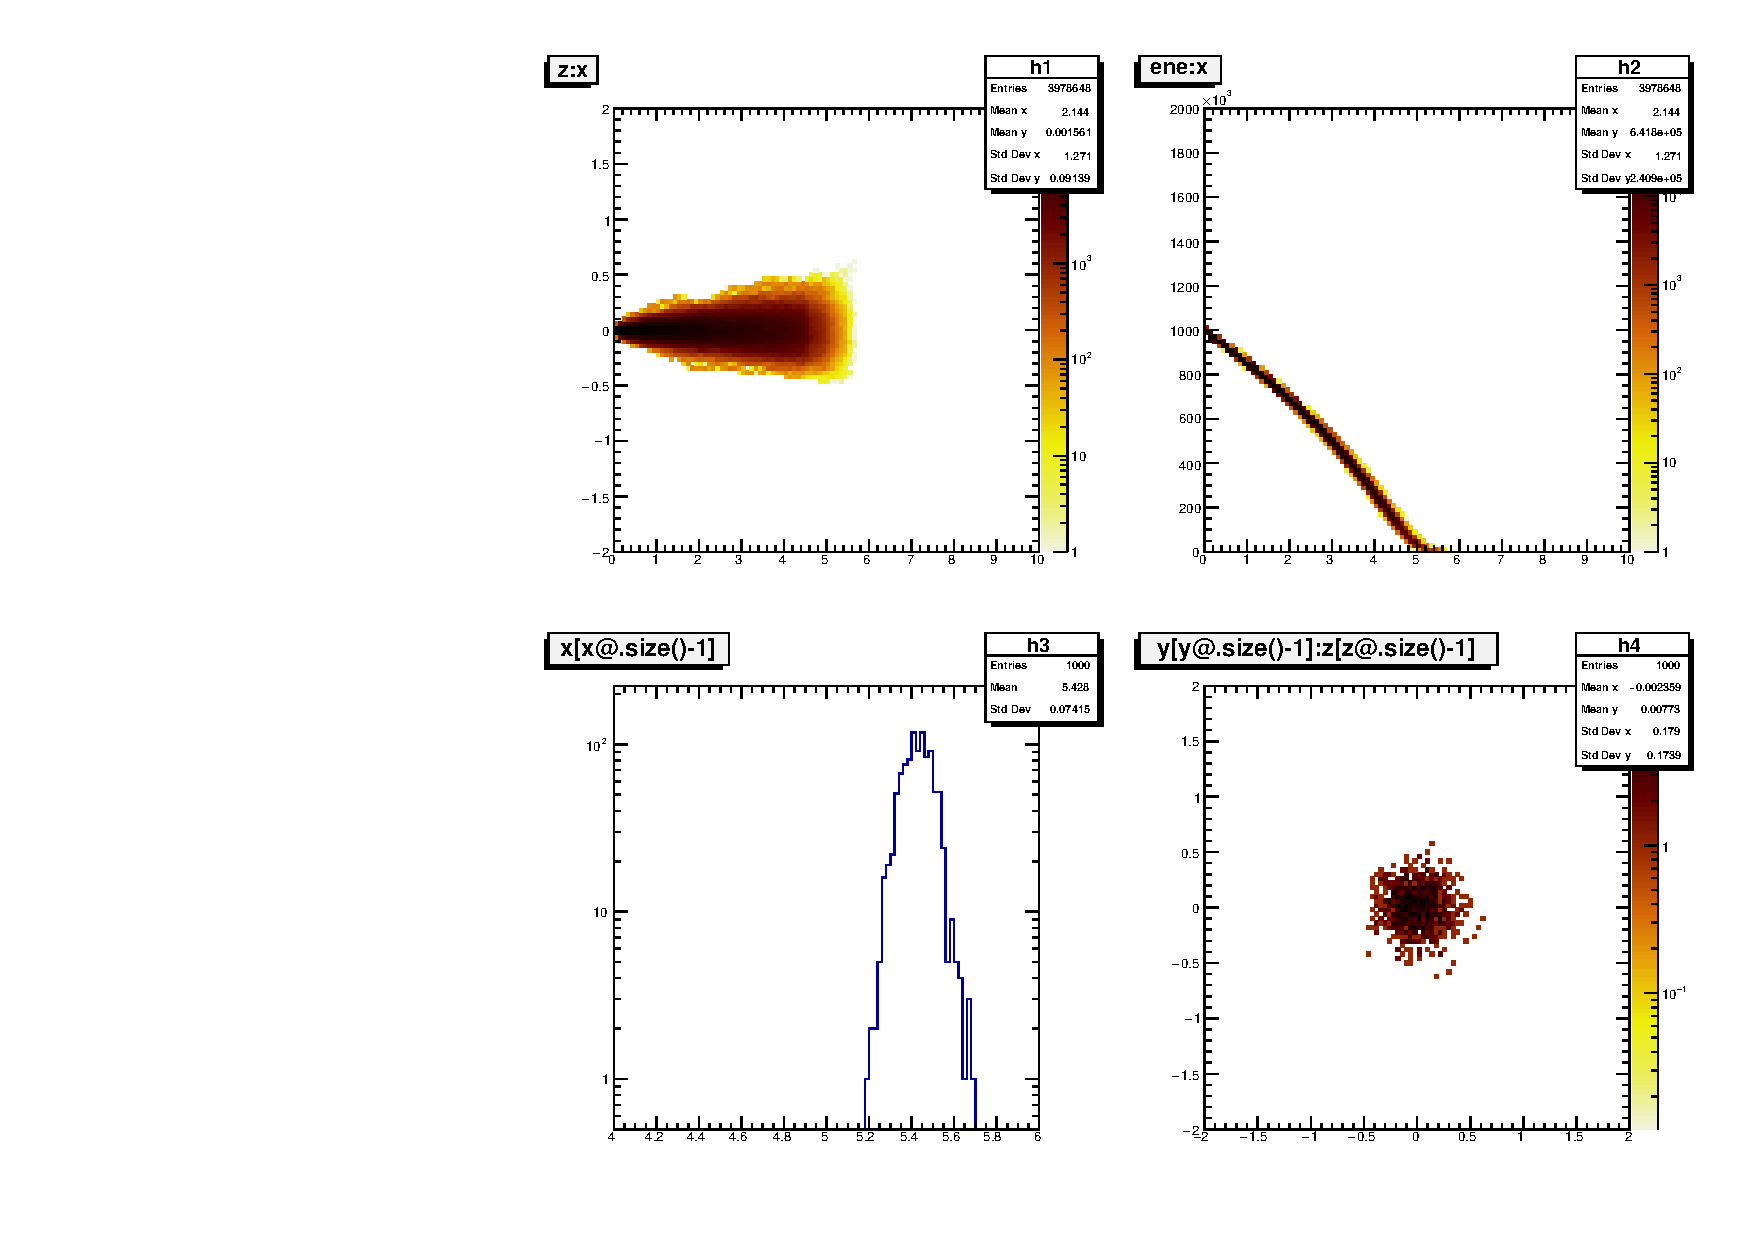
\includegraphics[width=\linewidth]{./pic/TrackSrim.pdf}
            \end{center}
        \end{minipage}
        &
        \begin{minipage}{0.45\linewidth}   
            \begin{center}
            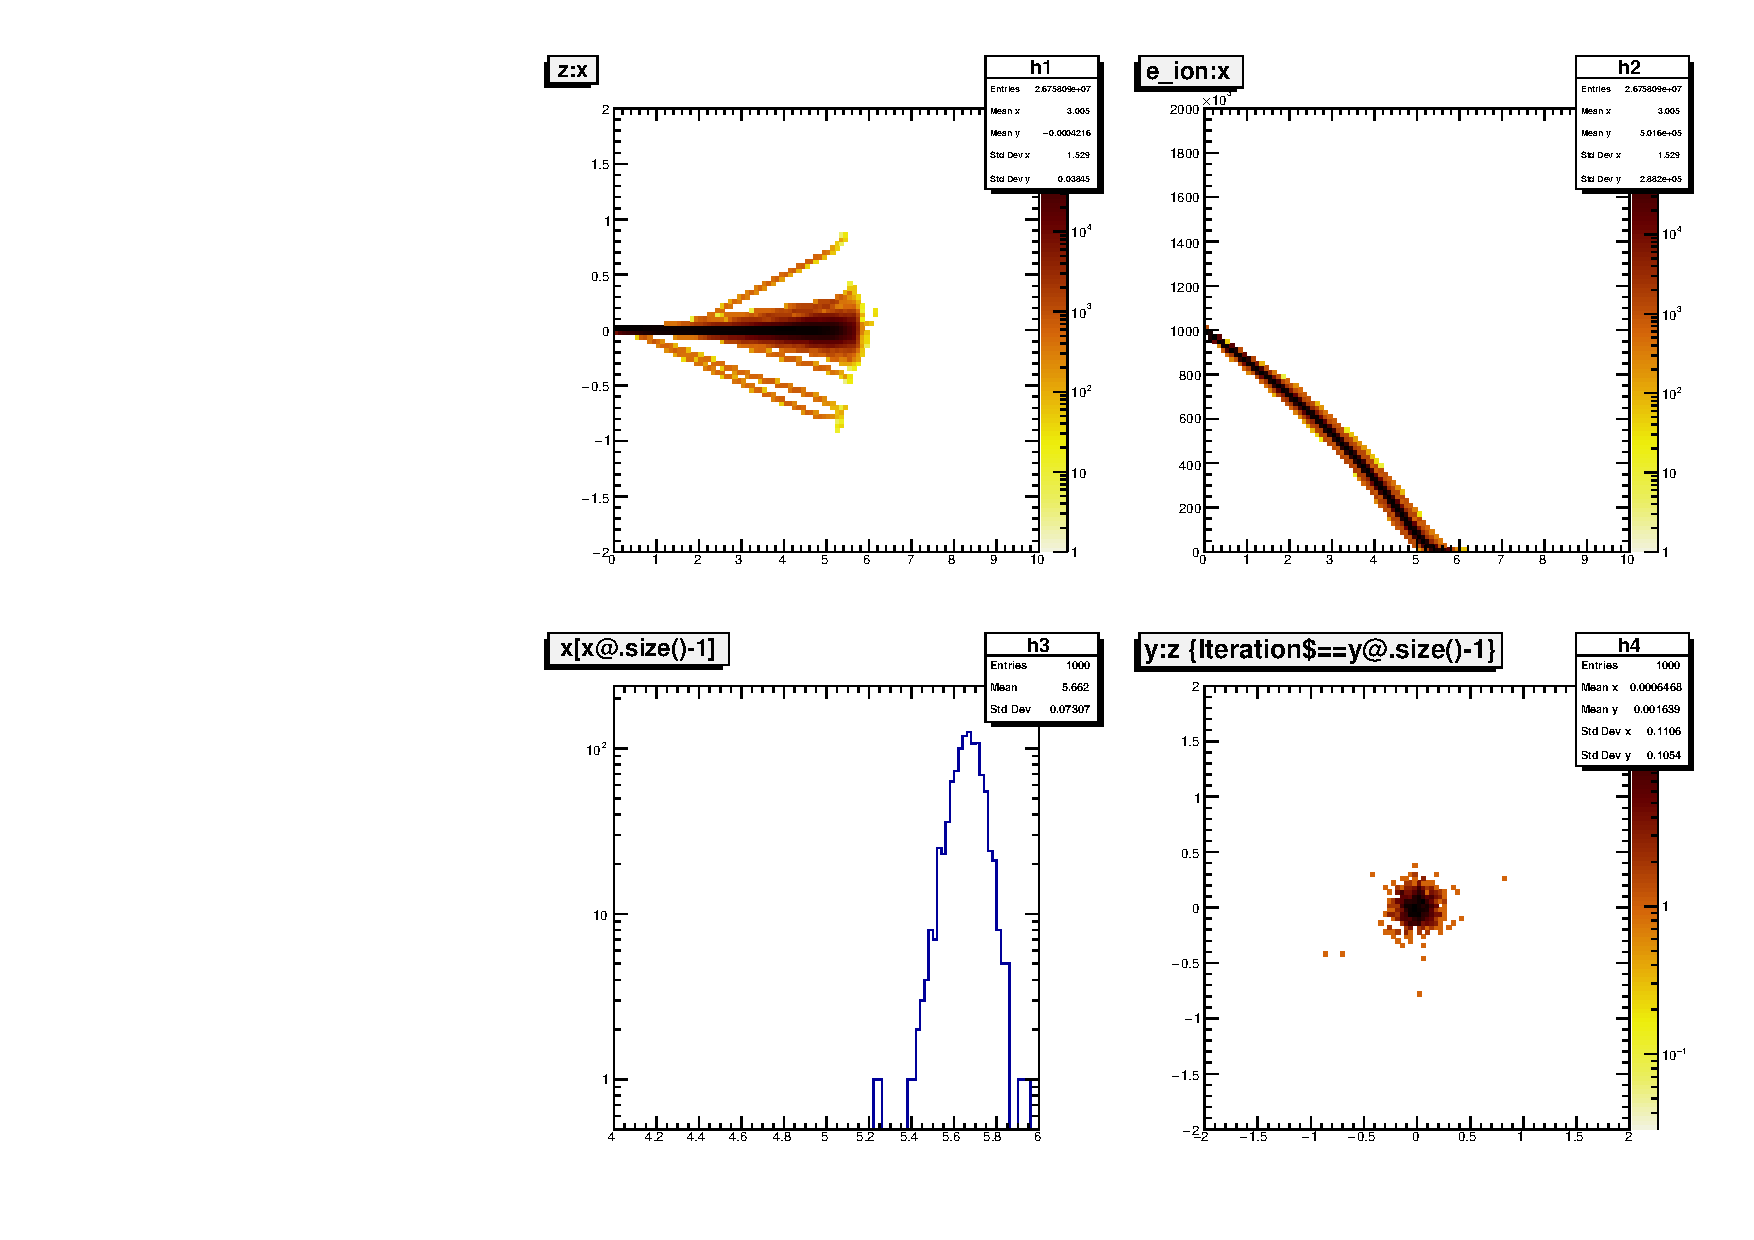
\includegraphics[width=\linewidth]{./pic/TrackTrimSQLite.pdf}
            \end{center}
        \end{minipage}
        \\
        \begin{minipage}{0.45\linewidth}   
            \begin{center}
            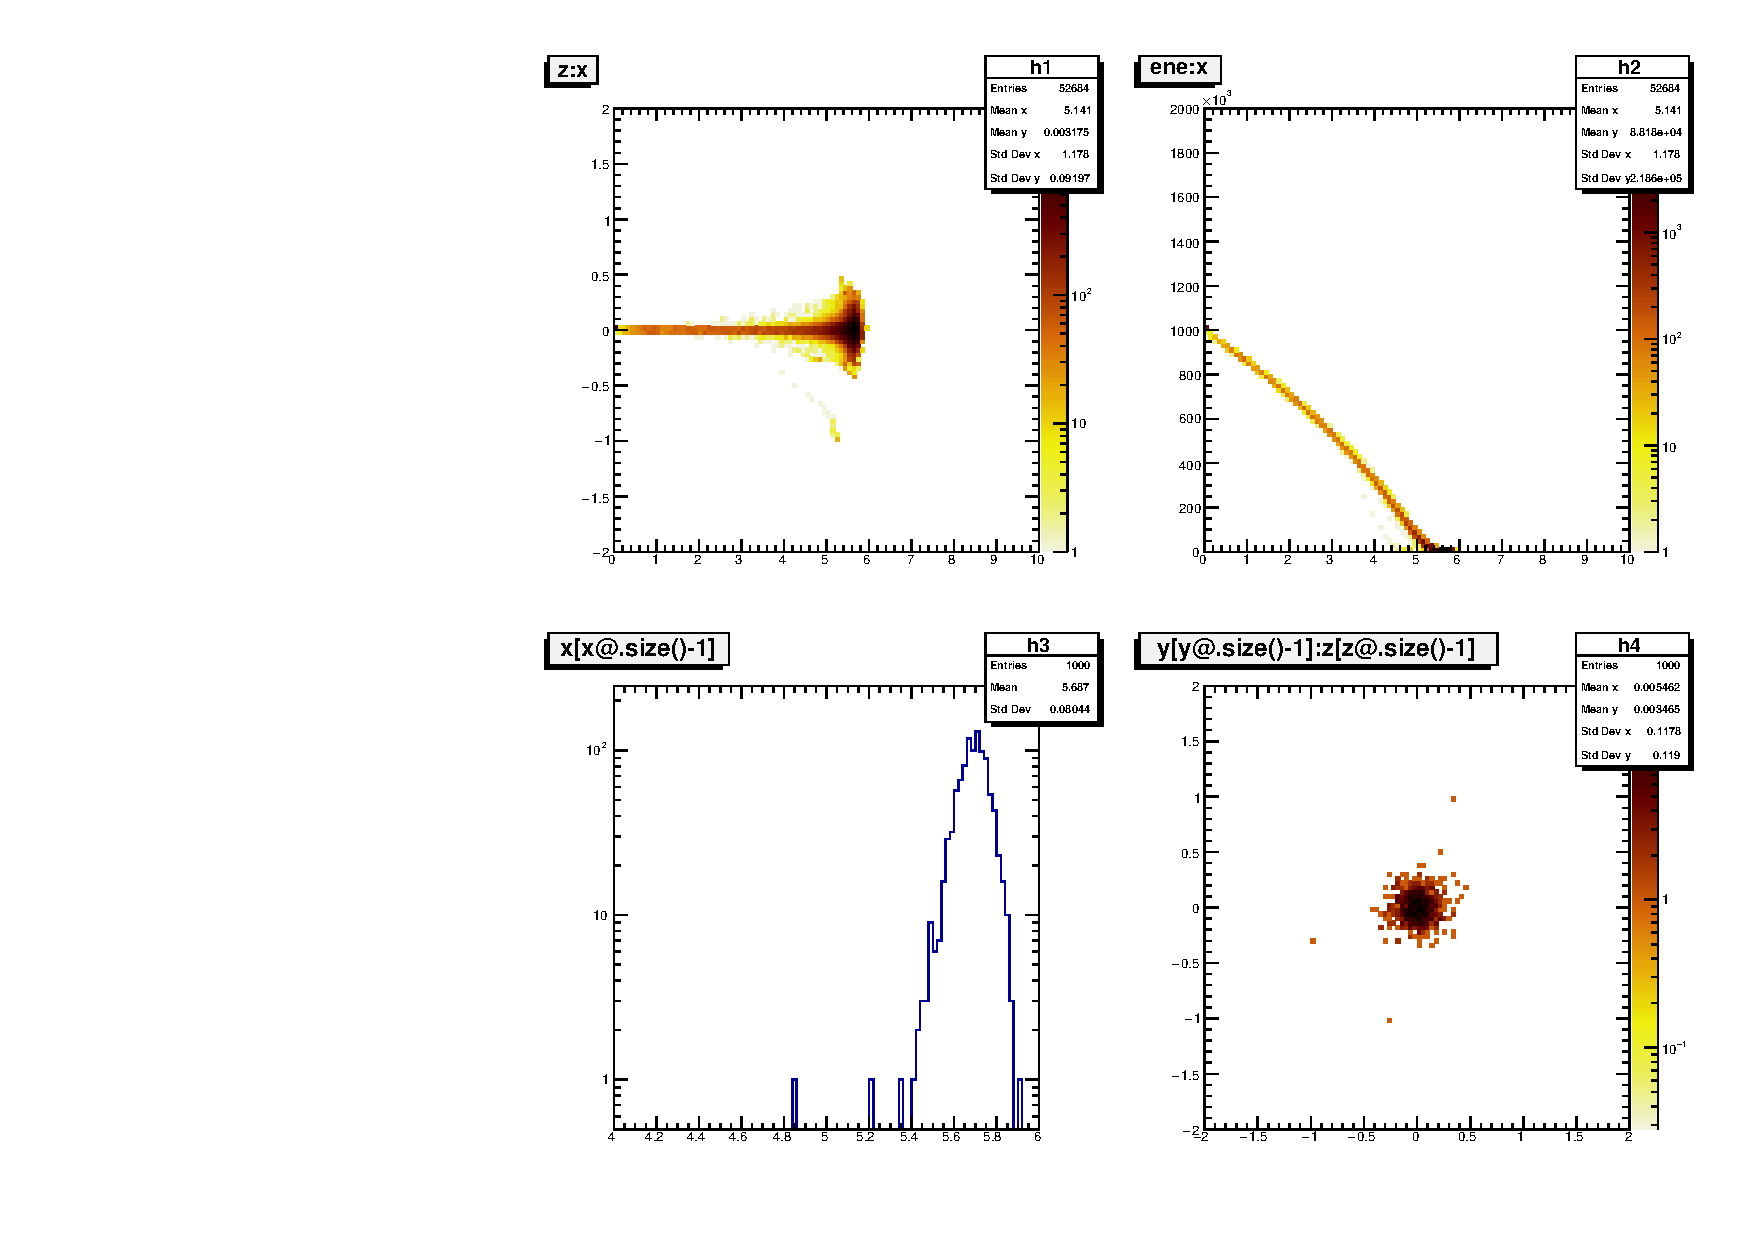
\includegraphics[width=\linewidth]{./pic/trim_raw.pdf}
            \end{center}
        \end{minipage}
    \end{tabular}
\end{center}
    \caption{生成した飛跡。4つのヒストグラムが一つの計算条件に対応する。左上がGarfield++のTrackSrim、右上が今回開発したTrackTrimSQLite、左下がTrackTrimSQLiteの入力に用いたTRIMの計算結果。詳細は本文参照。}
    \label{fig:reflectivity}
\end{figure}




\section{まとめ}
Garfield++の飛跡生成アルゴリズムの誤りを修正した新たなクラスTrackTrimSQLiteを開発した。
このクラスではTRIMの計算した飛跡の形状データをもとに新たな飛跡を生成する。
同一条件のシミュレーションを実行し、
TrackTrimSQliteの計算結果は飛跡の形状がTrackSrimとは異なり正しいと思われる形状をしていること、
TRIMの計算結果と同様の分布に従うことを確認した。

% \includepdf[pages=-,  noautoscale=true, scale=0.9, pagecommand={}]
%      {../../pdf/ComputerGenesis/early_stage.pdf}

\newpage

\appendix
\section{SRIM (The Stopping and Range of Ions in Matter)}
SRIMは物質中に侵入したイオンの阻止能や飛程を計算する一群のプログラムであり、
計算の過程ではイオンと物質中の原子の衝突過程は量子力学的に取り扱われる。
 (以下では移動する原子をイオンと呼び、標的中の原子を原子と呼称する。) 
SRIMの計算は統計的アルゴリズムを用いることで効率化されている。
まずイオンは連続する衝突点の間を離散的に移動する。
その後、衝突点の間の衝突の効果が平均化されて取り入れられる。
イオンと原子の衝突過程としては、電子の交換と重なり合う電子殻同士の相互作用などの過程を含む
遮蔽されたポテンシャルによるクーロン散乱を考慮する。
その他に、イオンは電子の励起やプラズモン生成を引き起こす長距離相互作用を行う。
これらの過程は、標的の集団的な電子的構造と原子間結合についての情報を取り入れることで
計算開始時に設定される。
標的中のイオンの荷電状態は実行電荷の考え方をもとに記述される。
この記述には、荷電状態の速度依存性や標的中の集団的な電子の海による長距離遮蔽効果も含まれる。

計算方法に関しての完全な記述は我々の書籍
 "SRIM - The Stopping and Range of Ions in Solids",
  by J. F. Ziegler and J. P. Biersack in 1985 (the Transport of Ions in Matter) 
に書かれている。
この本はイオンの固体への侵入過程の物理が単純な例によって示され、
その後SRIMのソースコードが物理過程の完全な説明とともに記述されている。
その後の章ではSRIMの正確性と応用事例が述べられる。
このウェブサイトでは、SRIMで計算して阻止能のプロットと
水素とヘリウムのイオンについての入手可能なすべての実験データをダウンロードすることができる。

TRIMはSRIMに含まれる最も包括的なプログラムである。
TRIMでは最大8層の混合物からなる複雑な形状の標的について計算を行うことができる。
このプログラムは
終状態におけるイオンの三次元的分布およびイオンのエネルギー損失に伴って発生する
標的損傷、スパッタリング、イオン化、フォノン生成といった
あらゆる運動過程における現象について計算する。
また標的原子の二次的な反応過程も詳細に追跡される。
このプログラムは計算過程を任意のタイミングで中断し、
またその後中断した時点から再開することができるように作られている。
計算結果のプロットは必要に応じて保存したり、計算中に画面に表示することができる。
 (保存された計算結果を可視化には5秒を要する。)

SRIMはj. P. Biersackによる
飛程計算アルゴリズム (J. P. Biersack and L. Haggmark, Nucl. Instr. and Meth., vol. 174, 257, 1980) 
とJ. F. Zieglerによる阻止能に関する理論 ("The Stopping and Range of Ions in Matter", volumes 2 - 6, Pergamon Press, 1977-1985)
が元になっている。
SRIMのバージョンによる違いはSRIMパッケージのVERSIONというファイルの中に記述されている。

SRIMのプログラムは1983年にDOSのプログラムとして始まり、1989年にWindowsに移植された。

もし、あなたがSRIMのプログラムを科学論文に用いた場合、著者に論文をメールで送ってほしい。
このことはSRIMの将来的なサポートのために役立つだろう。

{\bf 
以上、\url{http://www.srim.org/SRIM/SRIMINTRO.htm} の記述を翻訳した。
}

\section{SRIMのインストール方法}
\subsection{概要}
SRIMは、SRIM.exeとTRIM.exeという2つの計算コードを含んでいる。
後述する手順でSRIMをインストールするとSRIM.exeとTRIM.exeを利用できるようになる。

SR.exeは一様な物質中でのイオンのエネルギー損失過程の
平均に関する情報を計算することができる計算コードで、
TRIM.exeは多層の物質中でのイオンのエネルギー損失過程を
詳細に計算するコードである。

また、これらの他にSR.exeとTIN.exeという実行ファイルも含まれている。
SRIM.exeはSRIMやTRIMを起動するためのソフトウェアであるが、
あまり使用することはないと思われる。
TIN.exeはTRIMの入力ファイルを作成するためのソフトウェアである。


\subsection{ダウンロード}
SRIMは公式のウェブページ\url{http://www.srim.org/SRIM/SRIMLEGL.htm}からダウンロード可能である。
基本的にSRIM-2013 (Professional) をダウンロードすればよい。
ダウンロードされるファイルは "SRIM-2013.e" という名前である。
このファイルの拡張子をexeに変更して実行すると、SRIMのファイル群が展開される。


\subsection{Windows}
ファイル群を展開しただけでは、SRIMを正常に動作させることができない。
SRIMを使用すると、"RICHTX.OCX"などのプログラムがないことを示すポップアップウインドウが現れ
アプリケーションが終了する。
この問題に対処する方法はSRIMを展開したディレクトリの
"SRIM Setup Message.pdf"に書かれている。
このファイルの記述によれば
\begin{itemize}
    \item MSVBvm50.exe
    \item ComCtl32.ocx
    \item ComDlg.ocx
    \item MSFlxGrd.ocx
    \item RichtX32.ocx
    \item TabCtl32.ocx
    \item LineDraw.ttf
\end{itemize}
の7つのプログラムが必要とのことである。

基本的には、この文章のセットアップ法\#1に従い、
SRIMを展開したディレクトリ配下の"SRIM-Setup/SRIM-AutoSetup"内にある、
"SRIM-AutoSetup.exe"を管理者として実行していけばよい。


\subsection{Linux}
LinuxではWindowsを仮想的に動作させるソフトウェアのWine上でSRIMを使用する方法がある。
そのためにまずWineをインストールする。
Wineのインストール方法はOSに依存するため、ここでは述べないが
基本的にパッケージマネージャからインストールすることができる。

以下で述べる手順はこのような環境でのものである。
\begin{screen}[4]
    $[$quser@oxygen SRIM$]$\$ cat /etc/lsb-release \\
    DISTRIB\_ID=Ubuntu \\
    DISTRIB\_RELEASE=18.04 \\
    DISTRIB\_CODENAME=bionic \\
    DISTRIB\_DESCRIPTION="Ubuntu 18.04.5 LTS" \\
    $[$quser@oxygen SRIM$]$\$ which wine \\
    /usr/bin/wine \\
    %[quser@oxygen SRIM]\$ wine --version \\
    wine-3.0 (Ubuntu 3.0-1ubuntu1) 
\end{screen}

基本的にはWindowsの場合と同様に必要なファイルをインストールしていくことになる。
Wineがインストールされている環境ではコマンドラインで
\begin{screen}[4]
    \$ wine (実行ファイル)
\end{screen}
とすることで仮想Windows環境からそのファイルを実行することができる。

まず、任意の場所にSRIMをダウンロードする。以下では例えば、"~quser/opt/SRIM"とする。

\begin{screen}[4]
    \$ cd ~quser/opt/SRIM \\
    \$ wget \url{http://www.srim.org/SRIM/SRIM-2013-Pro.e} \\
    \$ mv SRIM-2013-Pro.e SRIM-2013-Pro.exe \\
    \$ wine SRIM-2013-Pro.exe 
\end{screen}
とするとポップアップウインドウが現れるので、
Extractで圧縮されているファイルを展開し、Doneで終了する。

\begin{figure}[H]
    \centering
    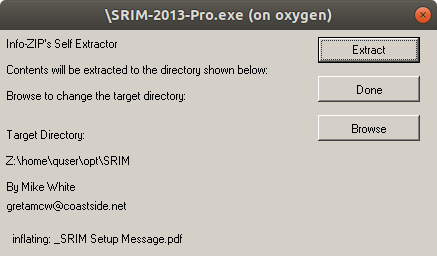
\includegraphics[width=10cm]{./pic/SRIM_extract.png}
    \caption{TRIMの入力ファイル生成用ソフトウェアTIN.exeの画面}
    \label{fig:reflectivity}
\end{figure}



その後必要なプログラムをインストールする。
Windowsの場合とは違って"Auto-Setup"がうまくできなかったので、
手動でプログラムをインストールする。
インストールすべきプログラムは、
SRIMのディレクトリ配下の"SRIM-Setup"に用意されているので、
以下の手順の前にそこに移動しておく。

\begin{screen}[4]
    \$ cd SRIM-Setup
\end{screen}

そして、Visual Studioのランタイムパッケージをインストールする。
\begin{screen}[4]
    \$ wine MSVBvm50.exe
\end{screen}
これを実行すると、図\ref{fig:VB_inquiry}のようなウインドウが現れるので、"Yes" を選択する。
インストールが終わると、図\ref{fig:VB_done}のようなウインドウが現れるので "OK" を選択し終了する。


\begin{figure}[H]
    \centering
    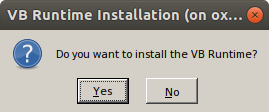
\includegraphics[width=10cm]{./pic/VB_runtime_inquiry.png}
    \caption{MSBvm50.exeのインストールを確認するポップアップウインドウ。}
    \label{fig:VB_inquiry}
\end{figure}

\begin{figure}[H]
    \centering
    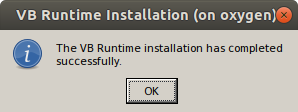
\includegraphics[width=10cm]{./pic/VB_runtime_done.png}
    \caption{MSBvm50.exeのインストール完了時にあらわれるポップアップウインドウ。}
    \label{fig:VB_done}
\end{figure}


最後に、必要なOCXファイルをインストールする。
\begin{screen}[4]
    \$ wine ../../../.wine/drive\_c/windows/syswow64/regsvr32.exe RichTx32.ocx \\
    \$ wine ../../../.wine/drive\_c/windows/syswow64/regsvr32.exe ComDlg32.ocx  \\
    \$ wine ../../../.wine/drive\_c/windows/syswow64/regsvr32.exe MSFlxGrd.ocx \\
    \$ wine ../../../.wine/drive\_c/windows/syswow64/regsvr32.exe ComCtl32.ocx \\
    \$ wine ../../../.wine/drive\_c/windows/syswow64/regsvr32.exe TabCtl32.ocx 
\end{screen}
これらのファイルのインストールが成功すると
\begin{screen}[4]
    regsvr32: Successfully registered DLL 'TabCtl32.ocx'
\end{screen}
というようなメッセージがかえってくる。

ここまでの手順を終えると、SRIMを展開したディレクトリで
\begin{screen}[4]
    \$ wine SRIM.exe
\end{screen}
などとすれば、SRIMやTRIMを使用することができるはずである。

% SRIMを使用するためには、
% Windowsでのインストールと同様に必要なプログラムを追加でwineの仮想環境にインストールする必要がある。
% それには完全に同じ方法で "SRIM-Setup" にある自動インストールツールを使っても良いかもしれないが
% この方法でインストールできるかどうかは未確認である。
% 以下では、手動で必要なプログラムをインストールする手順について述べる。
% この手順は手探りで発見したものであるので、おそらく様々な点で非効率的であるかもしれないことに
% 注意されたい。

% この手順では、まず\url{https://www.microsoft.com/en-us/download/details.aspx?id=24417}から

% \url{https://www.microsoft.com/ja-jp/download/details.aspx?id=5721}
% からVisual Basic Service Pack 6を、
% \url{https://www.microsoft.com/ja-jp/download/details.aspx?id=10019}から
% Microsoft Visual Basic 6.0 コモンコントロールをダウンロードする。
% 前者は"Vs6sp6B.exe"というファイルなので、
% \begin{screen}[4]
%     \$ wine Vs6sp6B.exe
% \end{screen}
% としてこれを実行する。
% 実行すると、ファイルを展開する場所を尋ねられるので
% 適当に指定する。
% 実行後、ファイルの展開先にある
% \begin{itemize}
%     \item RichTx32.CAB
%     \item MsFlxGrd.CAB
%     \item TabCtl32.CAB
%     \item Com
% \end{itemize}


\section{TRIMの使い方}
\subsection{入力ファイルの生成}
TRIMの計算条件はTRIMのインストール先ディレクトリにあるTRIM.INというテキストファイルに書き込む。
これを編集するためのアプリケーションがTIN.exeである。
TIN.exeの画面を図\ref{fig:TIN}に示す。

\begin{figure}[H]
    \centering
    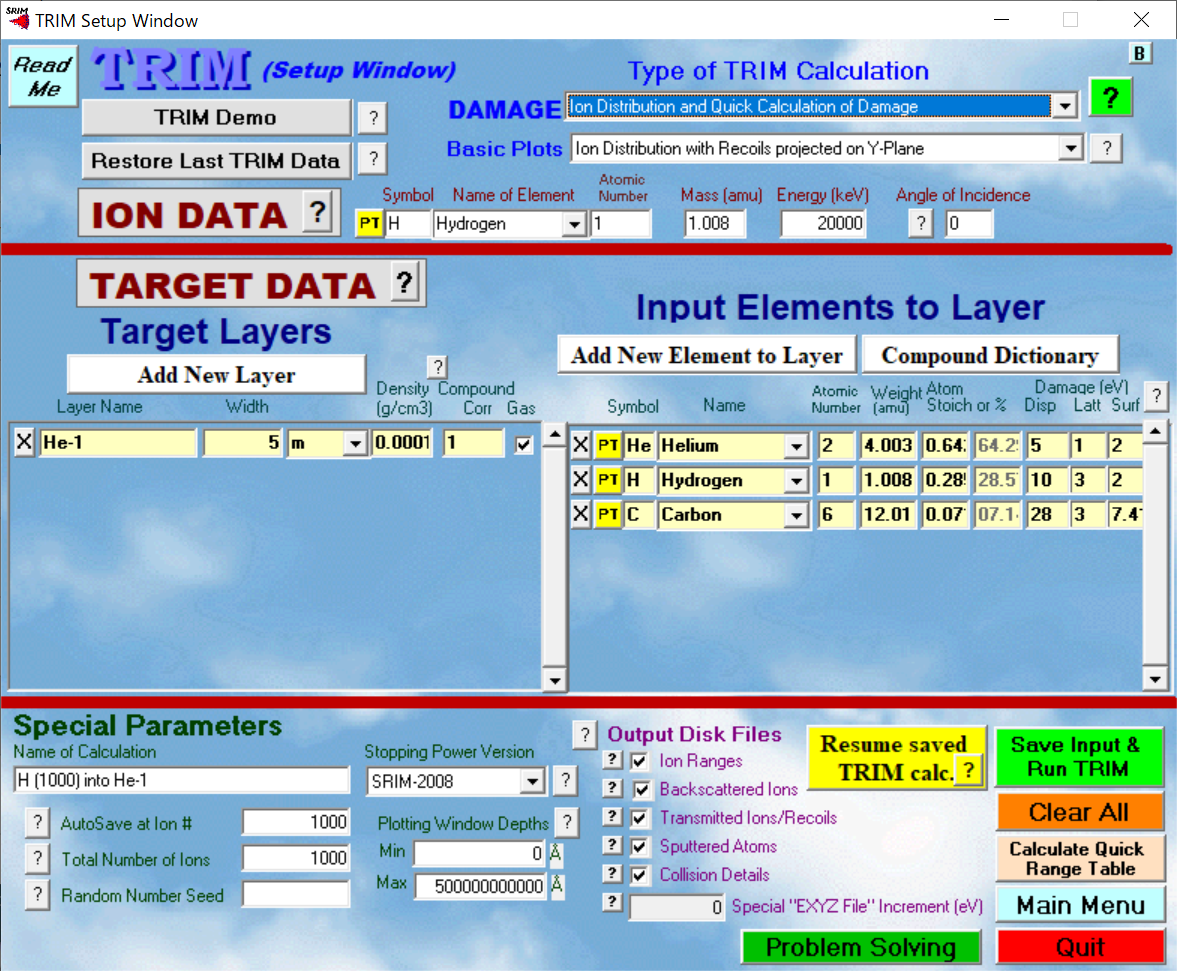
\includegraphics[width=10cm]{./pic/TIN.jpg}
    \caption{TRIMの入力ファイル生成用ソフトウェアTIN.exeの画面}
    \label{fig:TIN}
\end{figure}

TrackTrimSQLiteの入力として用いる場合、TIN.exeウインドウの右上 "DAMAGE" の項目を
”Ion Distribution and Quick Calculation of Damage”に設定して、
ウインドウ右下の "Output Disk Files" のすべてにチェックをしておく必要がある。
また、媒質の層の厚さを表す "Width" を粒子の飛程に比べて十分大きくしておく必要がある。

TIN.exeは日本語のWindows環境で頻繁に異常な動作を示す。
その一例として、数値を入力するためのフィールドが点滅し操作不能になることがある。
この場合、Win+dを二回続けて入力すると元の状態に復帰できる。
しかしこの異常は非常に頻繁に発生するので、TIN.exeを用いて入力ファイルを作成することは
推奨できない。
その代わりにテキストエディタからTRIM.INを直接編集し、
動作の確認のみをTIN.exeで行うほうが素早く入力ファイルを編集することができる。

生成されたTRIM.INを以下に示す。

\begin{lstlisting}[caption={TRIM.INの例。},basicstyle=\fontsize{6}{6}\ttfamily,identifierstyle=\fontsize{6}{6},numberstyle={\tiny},columns=fixed]
    ==> SRIM-2013.00 This file controls TRIM Calculations.
Ion: Z1 ,  M1,  Energy (keV), Angle,Number,Bragg Corr,AutoSave Number.
     1   1.008         20000       0    1000        1     1000
Cascades(1=No;2=Full;3=Sputt;4-5=Ions;6-7=Neutrons), Random Number Seed, Reminders
                      1                                   0       0
Diskfiles (0=no,1=yes): Ranges, Backscatt, Transmit, Sputtered, Collisions(1=Ion;2=Ion+Recoils), Special EXYZ.txt file
                          1       1           1       1               2                               0
Target material : Number of Elements & Layers
"H (1000) into He-1                      "       3               1
PlotType (0-5); Plot Depths: Xmin, Xmax(Ang.) [=0 0 for Viewing Full Target]
       0                         0           5E+11
Target Elements:    Z   Mass(amu)
Atom 1 = He =        2   4.003
Atom 2 = H =         1   1.008
Atom 3 = C =         6  12.011
Layer   Layer Name /               Width Density     He(2)    H(1)    C(6)
Numb.   Description                (Ang) (g/cm3)    Stoich  Stoich  Stoich
 1      "He-1"            5E+11  .000104   .6429   .2857   .0714
0  Target layer phases (0=Solid, 1=Gas)
1 
Target Compound Corrections (Bragg)
 1  
Individual target atom displacement energies (eV)
       5      10      28
Individual target atom lattice binding energies (eV)
       1       3       3
Individual target atom surface binding energies (eV)
       2       2    7.41
Stopping Power Version (1=2011, 0=2011)
 0 
\end{lstlisting}
実用的には同一ガス組成でいろいろな種類の粒子の飛跡を計算したいと思われる。
その場合、TRIM.INのガス組成さえ正しく設定しておけば、
TRIM.INの3行目で粒子の種類を、目的によっては18行目で粒子の変更するだけで良いと思われる。


\subsection{計算}
TRIMの計算はTRIM.exeを用いて行う。
TRIM.exeを実行するとTRIM.INを入力として直ちに計算が開始される。
図にTRIM.exeの実行中の画面を図\ref{fig:TRIM_calc}に示す。
計算が終了すると、図\ref{fig:TRIM_calc_end}のようにポップアップが現れる。
ポップアップするウインドウを拡大したものが図\ref{fig:TRIM_save}である。
ここで"はい"を選択して計算結果を保存する。
すると、保存先を尋ねる図\ref{fig:TRIM_save_directory}のようなウインドウが現れる。
ここで”Store in SRIM directory”を選択すると
結果のテキストファイルはSRIMのディレクトリの下にある"SRIM Outputs"に保存される。

計算結果ファイルの最終行で正しく終端処理を行うためにはTRIMのウインドウを閉じる必要がある。
TRIMのウインドウの右上のバツボタンを押すと、図\ref{fig:TRIM_save_status}のようなウインドウが現れる。
計算結果を使うだけであればどちらを選んでも差し支えない。

\begin{figure}[H]
    \centering
    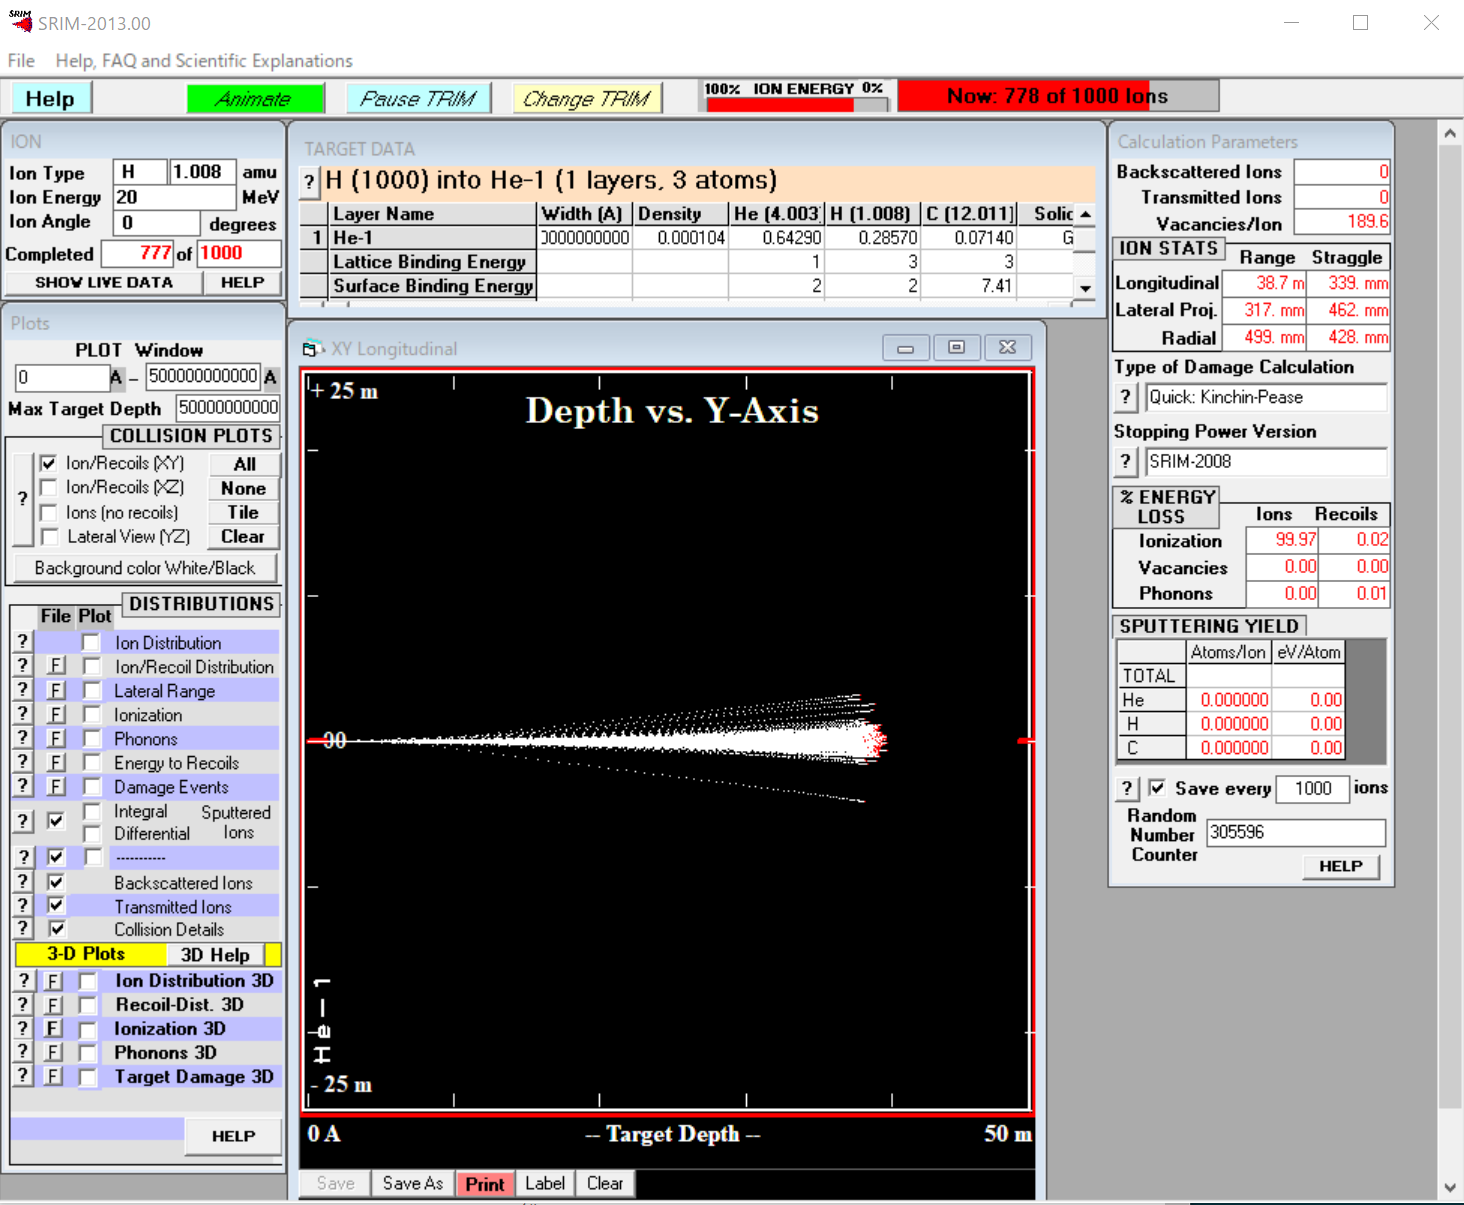
\includegraphics[width=12cm]{./pic/TRIM_calc.jpg}
    \caption{TRIMの計算途中の様子。計算の進行とともに右上のプログレスバーが右に動いている。}
    \label{fig:TRIM_calc}
\end{figure}


\begin{figure}[H]
    \centering
    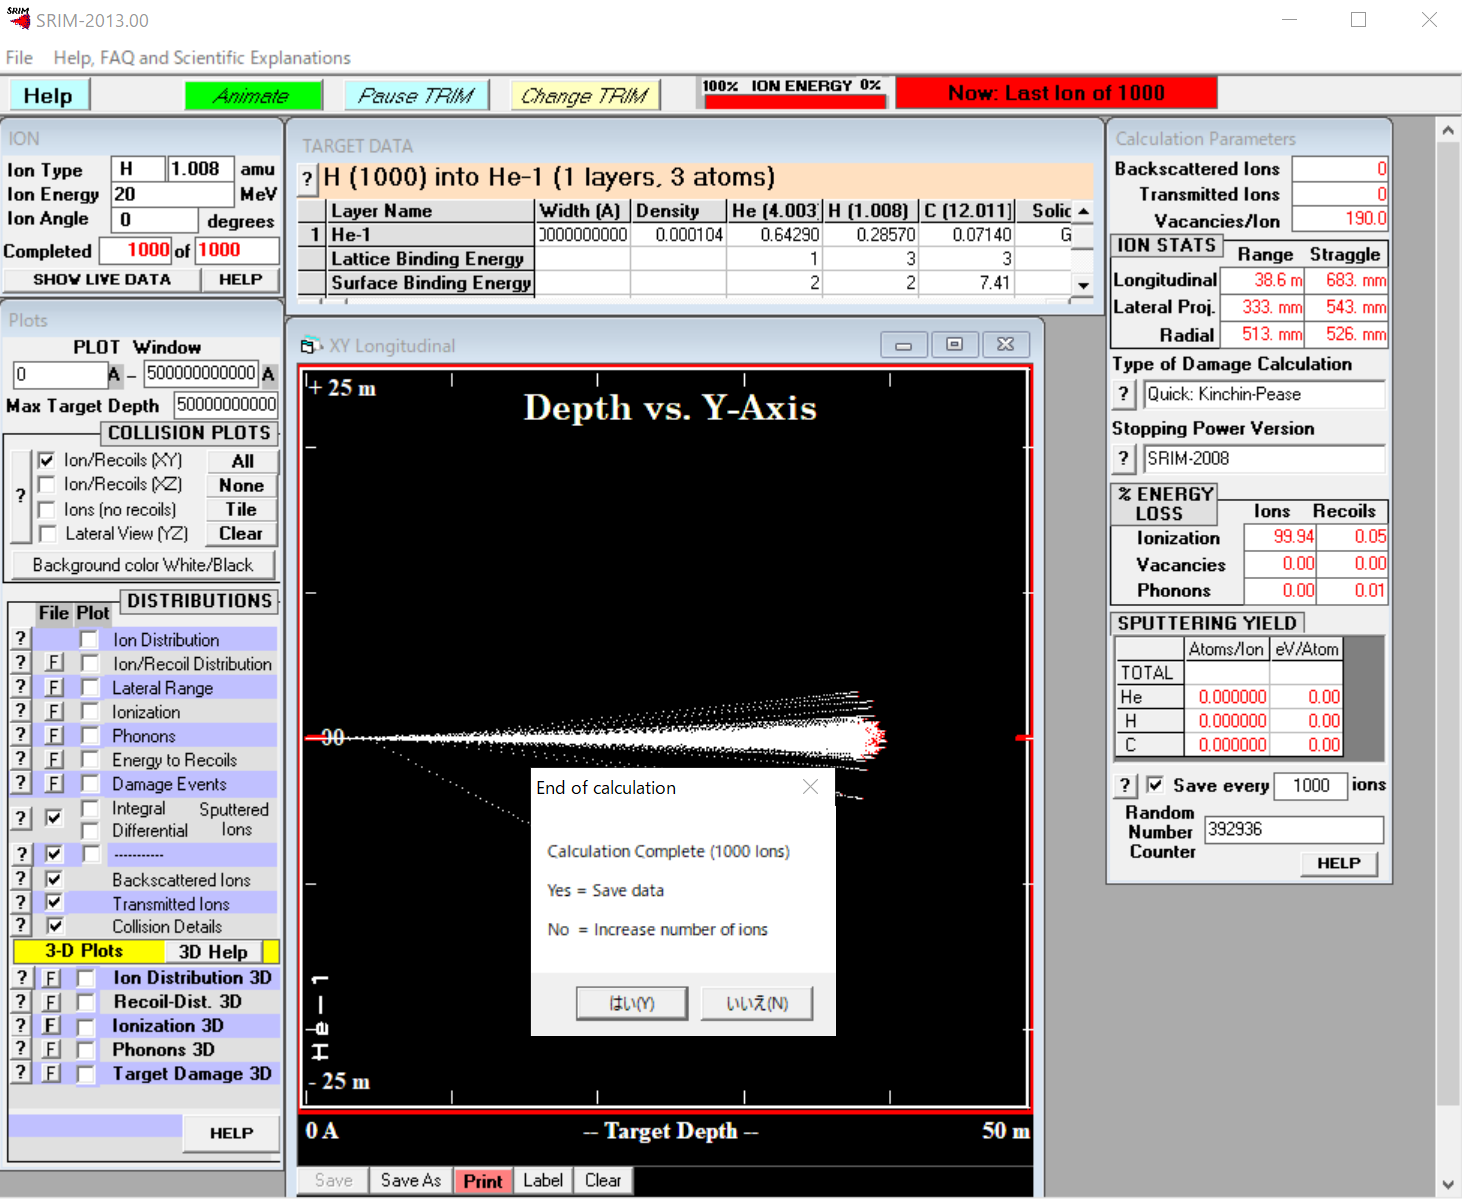
\includegraphics[width=12cm]{./pic/TRIM_calc_end.jpg}
    \caption{TRIMの計算終了時の様子。計算後の処理を尋ねるウインドウがポップアップする。}
    \label{fig:TRIM_calc_end}
\end{figure}


\begin{figure}[H]
    \centering
    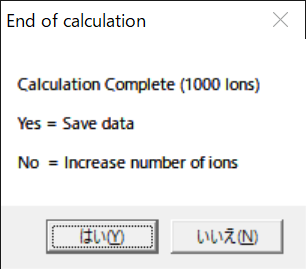
\includegraphics[width=10cm]{./pic/TRIM_save.jpg}
    \caption{TRIMの計算終了時にポップアップするウインドウ。"はい"を選択し、計算結果を保存する。}
    \label{fig:TRIM_save}
\end{figure}


\begin{figure}[H]
    \centering
    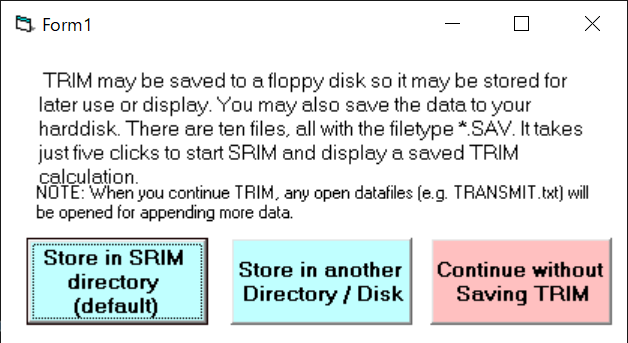
\includegraphics[width=10cm]{./pic/TRIM_save_directory.jpg}
    \caption{TRIM計算結果の保存先ディレクトリを指定するためのウインドウ。
    図\ref{fig:TRIM_save}で計算結果を保存することを選択するとポップアップする。}
    \label{fig:TRIM_save_directory}
\end{figure}


\begin{figure}[H]
    \centering
    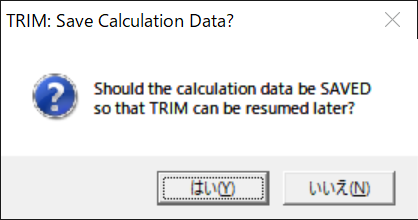
\includegraphics[width=10cm]{./pic/TRIM_save_status.jpg}
    \caption{TRIMのウインドウを右上のバツボタンで閉じるときに現れるウインドウ。
    "いいえ"を選択して問題ない。}
    \label{fig:TRIM_save_status}
\end{figure}




\section{TRIMの出力ファイルの形式}
TRIMでは計算結果をいくつかのテキストファイルに保存することができる。
以下ではTrackTrimSQLiteの入力ファイルを作るために必要な
2つのファイルCOLLISON.txtとRANGE\_3D.txtについて述べる。
\subsection{COLLISON.txt}
COLLISON.txtはイオンの物質中での衝突事象を記録している。
なお、COLLISON.txtの形式は指定したTRIMの計算モデルによって変わるが、
TrackTRIMSQLiteが対応する形式は "DAMAGE" として "Ion Distribution and Quick Calculation of Damage"を選んだフォーマットである。

リストにCOLLISON.txtの例を示す。
COLLISON.txtのはじめには計算条件を記録しているヘッダーがあり、
その後各イベントの衝突履歴が示されている。
リストの35行目以降の各行が一つの衝突に対応しており、
値の凡例は34行目にある。
各行をよく観察するとすべての行の同じ列に数字の3がつらなっていることがわかる。
これは、なぜか区切り文字が数字の3になっているためであると思われる。

衝突事象を記述する値の読み取り方を最初の衝突事象の35行目を一例として解説する。
区切り文字3に注目すると、この行の衝突事象はイオン番号が1、エネルギーが98.22E+02 (keV)、
深さが62396.E+04 (\AA)、yが-2698.E-03 (\AA)、zが1889.E-03 (\AA)、Seが0 (eV/A)、
衝突した原子がHe、反跳エネルギーが80472.E-04 (eV) とわかる。
a


\begin{lstlisting}[caption={COLLISION.txtの例。1イベントのみ抽出。},basicstyle=\fontsize{6}{6}\ttfamily,identifierstyle=\fontsize{6}{6},numberstyle={\tiny},columns=fixed]
============================== SRIM-2013.00 ==============================
==============================================================================
------------------------------------------------------------------------------
====== TRIM Calc.=  H(10 MeV) ==> He-1(  3 m) ================================
------------------------------------------------------------------------------
============================================================
o     Ion Name   =      H                                  o
o     Ion Mass   =    003.016 amu                          o
o     Ion Energy =000010000.0 keV                          o
============================================================
>     He  Displacement Energy of He = 0005.00000 eV
  Latt.Binding Energy of He = 0001.00000 eV
  SurfaceBind. Energy of He = 0002.00000 eV
>      H  Displacement Energy of  H = 0010.00000 eV
  Latt.Binding Energy of  H = 0003.00000 eV
  SurfaceBind. Energy of  H = 0002.00000 eV
>      C  Displacement Energy of  C = 0028.00000 eV
  Latt.Binding Energy of  C = 0003.00000 eV
  SurfaceBind. Energy of  C = 0007.41000 eV
============================================================
==========================================================================
3=> Recoils Calculated with Kinchin-Pease Theory (Only Vacancies Calc) <=3
==========================================================================
 
==========================  COLLISION HISTORY  =======================================================
  NOTES: Only Ion Collisions which produce Displacements are tabulated.                               
         Atom Sums and Averages are Incomplete if Recoil Cascades Leave Target.                       
         Target DISPlacements = VACancies + REPLACement Collisions.                                   
         Target VACancies = INTERstitials + Sputtered + Transmitted Atoms.                            
                            Recoil Atoms which end at the surface, are not counted (see manual).      
======================================================================================================
  Ion    Energy    Depth     Lateral Distance (A)   Se    Atom  Recoil    Target Target Target Target 
  Numb   (keV)      (A)       Y Axis    Z Axis    (eV/A)  Hit  Energy(eV) DISP.  VAC.   REPLAC INTER  
------------------------------------------------------------------------------------------------------
300001398.44E+02362396.E+043-2698.E-033 1889.E-0330000.003 He 380472.E-043000000001.0003      3      3
300001396.93E+02312230.E+053 5829.E+023-2228.E+0230000.003 He 314007.E-033000000001.0003      3      3
300001394.59E+02320912.E+053 2572.E+033-1754.E+0230000.003  C 310852.E-023000000001.1543      3      3
300001390.24E+02337691.E+053 1053.E+043 1369.E+0430000.003 He 328631.E-033000000001.8753      3      3
300001387.97E+02345808.E+053 1412.E+043 2032.E+0430000.003 He 311376.E-033000000001.0003      3      3
300001383.64E+02361476.E+053 1959.E+043 3192.E+0430000.003 He 311216.E-033000000001.0003      3      3
300001381.51E+02369033.E+053 2225.E+043 3840.E+0430000.003 He 335646.E-033000000002.3083      3      3
300001379.34E+02376408.E+053 2643.E+043 4393.E+0430000.003 He 310326.E-033000000001.0003      3      3
300001377.24E+02383599.E+053 2958.E+043 4952.E+0430000.003 He 315785.E-033000000001.0613      3      3
300001375.23E+02390612.E+053 3183.E+043 5416.E+0430000.003 He 368992.E-033000000004.2793      3      3
300001373.05E+02397454.E+053 3166.E+043 5846.E+0430000.003 He 316842.E-033000000001.1293      3      3
300001369.03E+02311059.E+063 3304.E+043 6658.E+0430000.003 He 361495.E-043000000001.0003      3      3
300001367.01E+02311690.E+063 3481.E+043 6966.E+0430000.003 He 310805.E-033000000001.0003      3      3
300001362.77E+02312900.E+063 4169.E+043 7678.E+0430000.003  H 366835.E-033000000002.0783      3      3
300001360.81E+02313477.E+063 4620.E+043 8183.E+0430000.003 He 364959.E-043000000001.0003      3      3
300001356.63E+02314580.E+063 5370.E+043 9142.E+0430000.003 He 370799.E-043000000001.0003      3      3
300001354.56E+02315104.E+063 5736.E+043 9517.E+0430000.003  H 317956.E-033000000001.0003      3      3
300001352.62E+02315611.E+063 6086.E+043 9932.E+0430000.003 He 393246.E-043000000001.0003      3      3
300001350.60E+02316100.E+063 6477.E+043 1039.E+0530000.003 He 311900.E-033000000001.0003      3      3
300001348.60E+02316572.E+063 6893.E+043 1090.E+0530000.003 He 314230.E-033000000001.0003      3      3
300001346.54E+02317027.E+063 7375.E+043 1136.E+0530000.003 He 310430.E-033000000001.0003      3      3
300001344.53E+02317464.E+063 7895.E+043 1175.E+0530000.003  H 312117.E-033000000001.0003      3      3
300001342.59E+02317883.E+063 8385.E+043 1208.E+0530000.003 He 322864.E-033000000001.5133      3      3
300001336.77E+02319038.E+063 9983.E+043 1324.E+0530000.003 He 385278.E-043000000001.0003      3      3
300001334.81E+02319389.E+063 1046.E+053 1364.E+0530000.003 He 390462.E-043000000001.0003      3      3
300001333.00E+02319722.E+063 1095.E+053 1408.E+0530000.003  C 375373.E-033000000001.0003      3      3
300001331.11E+02320039.E+063 1163.E+053 1470.E+0530000.003 He 366170.E-043000000001.0003      3      3
300001329.34E+02320339.E+063 1228.E+053 1524.E+0530000.003 He 310721.E-033000000001.0003      3      3
300001327.45E+02320624.E+063 1295.E+053 1574.E+0530000.003 He 342036.E-033000000002.6973      3      3
300001325.59E+02320892.E+063 1348.E+053 1617.E+0530000.003 He 323175.E-033000000001.5333      3      3
300001323.87E+02321142.E+063 1393.E+053 1649.E+0530000.003  H 331433.E-033000000001.0243      3      3
300001322.08E+02321378.E+063 1434.E+053 1674.E+0530000.003  H 315810.E-033000000001.0003      3      3
300001320.28E+02321597.E+063 1473.E+053 1695.E+0530000.003  C 351155.E-023000000004.1603      3      3
300001318.57E+02321799.E+063 1488.E+053 1654.E+0530000.003  C 366985.E-033000000001.0003      3      3
300001316.84E+02321986.E+063 1480.E+053 1608.E+0530000.003 He 346258.E-033000000002.9503      3      3
300001315.20E+02322157.E+063 1484.E+053 1566.E+0530000.003 He 391076.E-043000000001.0003      3      3
300001313.53E+02322313.E+063 1484.E+053 1531.E+0530000.003  H 387675.E-033000000002.6653      3      3
300001311.92E+02322453.E+063 1490.E+053 1497.E+0530000.003 He 313175.E-033000000001.0003      3      3
300001310.34E+02322577.E+063 1494.E+053 1462.E+0530000.003 He 314706.E-033000000001.0003      3      3
300001388.25E+01322687.E+063 1492.E+053 1429.E+0530000.003 He 393978.E-043000000001.0003      3      3
300001373.77E+01322782.E+063 1494.E+053 1401.E+0530000.003 He 331347.E-033000000002.0443      3      3
300001360.31E+01322863.E+063 1501.E+053 1374.E+0530000.003 He 320743.E-033000000001.3783      3      3
300001347.93E+01322930.E+063 1504.E+053 1355.E+0530000.003  H 326870.E-033000000001.0003      3      3
300001336.05E+01322986.E+063 1505.E+053 1340.E+0530000.003 He 323223.E-033000000001.5363      3      3
300001325.95E+01323028.E+063 1507.E+053 1324.E+0530000.003 He 315798.E-033000000001.0613      3      3
300001317.93E+01323060.E+063 1507.E+053 1315.E+0530000.003 He 318064.E-033000000001.2073      3      3
300001312.15E+01323084.E+063 1507.E+053 1306.E+0530000.003 He 312918.E-033000000001.0003      3      3
300001383.81E+00323100.E+063 1509.E+053 1298.E+0530000.003 He 311847.E-033000000001.0003      3      3
300001356.99E+00323113.E+063 1511.E+053 1291.E+0530000.003 He 348366.E-023000000022.3573      3      3
300001340.17E+00323121.E+063 1512.E+053 1276.E+0530000.003 He 312957.E-033000000001.0003      3      3
300001329.45E+00323128.E+063 1511.E+053 1265.E+0530000.003 He 344760.E-033000000002.8613      3      3
300001324.27E+00323133.E+063 1512.E+053 1255.E+0530000.003 He 322432.E-033000000001.4863      3      3
300001319.16E+00323137.E+063 1513.E+053 1244.E+0530000.003 He 317112.E-033000000001.1463      3      3
300001316.13E+00323141.E+063 1512.E+053 1236.E+0530000.003 He 334851.E-033000000002.2593      3      3
300001313.23E+00323144.E+063 1511.E+053 1230.E+0530000.003 He 323355.E-033000000001.5443      3      3
300001311.90E+00323146.E+063 1511.E+053 1226.E+0530000.003 He 323969.E-033000000001.5833      3      3
300001310.75E+00323149.E+063 1511.E+053 1221.E+0530000.003  H 347450.E-033000000001.5113      3      3
300001399.01E-01323151.E+063 1509.E+053 1217.E+0530000.003 He 362458.E-033000000003.9033      3      3
300001392.77E-01323153.E+063 1507.E+053 1214.E+0530000.003 He 318116.E-033000000001.2113      3      3
300001389.84E-01323155.E+063 1504.E+053 1213.E+0530000.003 He 390431.E-033000000005.4833      3      3
300001387.43E-01323157.E+063 1502.E+053 1214.E+0530000.003 He 349887.E-033000000003.1663      3      3
300001376.43E-01323159.E+063 1501.E+053 1217.E+0530000.003  C 349210.E-033000000001.0003      3      3
300001374.51E-01323161.E+063 1499.E+053 1222.E+0530000.003 He 336357.E-033000000002.3523      3      3
300001368.80E-01323163.E+063 1499.E+053 1226.E+0530000.003 He 323683.E-033000000001.5653      3      3
300001363.28E-01323164.E+063 1498.E+053 1232.E+0530000.003 He 376364.E-033000000004.6983      3      3
300001352.59E-01323166.E+063 1498.E+053 1238.E+0530000.003 He 320637.E-033000000001.3723      3      3
300001345.32E-01323167.E+063 1498.E+053 1245.E+0530000.003 He 323606.E-033000000001.5603      3      3
300001338.12E-01323168.E+063 1499.E+053 1250.E+0530000.003 He 313463.E-033000000001.0003      3      3
300001332.35E-01323169.E+063 1500.E+053 1254.E+0530000.003 He 352448.E-033000000003.3183      3      3
300001328.92E-01323170.E+063 1501.E+053 1256.E+0530000.003  H 313565.E-033000000001.0003      3      3
300001328.79E-01323171.E+063 1502.E+053 1259.E+0530000.003 He 313277.E-033000000001.0003      3      3
300001328.66E-01323172.E+063 1502.E+053 1261.E+0530000.003 He 331558.E-033000000002.0573      3      3
300001328.34E-01323172.E+063 1503.E+053 1264.E+0530000.003 He 326621.E-033000000001.7503      3      3
300001328.07E-01323173.E+063 1502.E+053 1267.E+0530000.003  C 342912.E-033000000001.0003      3      3
300001323.82E-01323174.E+063 1503.E+053 1271.E+0530000.003  H 377786.E-033000000002.3893      3      3
300001320.21E-01323174.E+063 1505.E+053 1274.E+0530000.003  H 315967.E-033000000001.0003      3      3
300001318.09E-01323175.E+063 1507.E+053 1278.E+0530000.003 He 368282.E-033000000004.2393      3      3
300001315.22E-01323176.E+063 1510.E+053 1280.E+0530000.003  H 330125.E-033000000001.0003      3      3
300001314.92E-01323176.E+063 1513.E+053 1282.E+0530000.003 He 363713.E-033000000003.9763      3      3
300001314.28E-01323176.E+063 1516.E+053 1284.E+0530000.003 He 349202.E-033000000003.1263      3      3
300001313.79E-01323177.E+063 1520.E+053 1285.E+0530000.003  H 379719.E-033000000002.4443      3      3
300001312.99E-01323177.E+063 1524.E+053 1286.E+0530000.003 He 318979.E-033000000001.2663      3      3
300001312.20E-01323177.E+063 1527.E+053 1287.E+0530000.003  H 335550.E-023000000008.8433      3      3
300001376.86E-02323177.E+063 1530.E+053 1288.E+0530000.003 He 312382.E-023000000007.2743      3      3
300001354.27E-02323178.E+063 1536.E+053 1287.E+0530000.003  H 311047.E-023000000003.2843      3      3
300001338.93E-02323178.E+063 1538.E+053 1286.E+0530000.003 He 319792.E-033000000001.3183      3      3
300001336.07E-02323178.E+063 1540.E+053 1286.E+0530000.003  H 399806.E-033000000002.9983      3      3
300001326.09E-02323178.E+063 1541.E+053 1285.E+0530000.003 He 316816.E-033000000001.1273      3      3
300001324.41E-02323178.E+063 1542.E+053 1283.E+0530000.003 He 340956.E-033000000002.6313      3      3
300001318.47E-02323178.E+063 1542.E+053 1282.E+0530000.003  H 349992.E-033000000001.5863      3      3
300001313.47E-02323178.E+063 1543.E+053 1281.E+0530000.003  H 320386.E-033000000001.0003      3      3
300001310.45E-02323178.E+063 1543.E+053 1280.E+0530000.003 He 324991.E-033000000001.6473      3      3
300001379.54E-03323178.E+063 1543.E+053 1279.E+0530000.003 He 383225.E-043000000001.0003      3      3
300001365.31E-03323178.E+063 1543.E+053 1279.E+0530000.003 He 317702.E-033000000001.1843      3      3
300001345.17E-03323178.E+063 1543.E+053 1278.E+0530000.003 He 327067.E-033000000001.7773      3      3
======================================================================================================
- For Ion 0000001:               For All Ions to date :                                              o
- Displacements     = 000000.0   Average Displacements/Ion     = 0000000.000                         o
- Replacements      = 000000.0   Average Replacements/Ion      = 0000000.000                         o
- Vacancies         = 000194.9   Average Vacancies/Ion         = 0000194.900                         o
- Interstitials     = 000000.0   Average Interstitials/Ion     = 0000000.000                         o
- Sputtered Atoms   = 000000.0   Average Sputter Atoms/Ion     = 0000000.000                         o
- Transmitted Atoms = 000000.0   Average Transmitted Atoms/Ion = 0000000.000                         o
======================================================================================================
  Ion    Energy    Depth     Lateral Distance (A)   Se    Atom  Recoil    Target Target Target Target 
  Numb   (keV)      (A)       Y Axis    Z Axis    (eV/A)  Hit  Energy(eV) DISP.  VAC.   REPLAC INTER  
------------------------------------------------------------------------------------------------------
\end{lstlisting}

\subsection{RANGE\_3D.txt}
RANGE\_3D.txtには生成された飛跡の終端位置の三次元座標が記録されている。
リストの20行目以降の各行が一つの飛跡に対応する。
イオンの通し番号はCOLLISON.txtを共通である。

\begin{lstlisting}[caption={RANGE\_3D.txtの例。5イベントを抽出。},basicstyle=\fontsize{6}{6}\ttfamily,identifierstyle=\fontsize{6}{6},numberstyle={\tiny},columns=fixed]
    ============================== SRIM-2013.00 ==============================
    ==============================================================================
    ====== SRIM Outputs\RANGE_3D.txt : File of Final Ion Positions =====
    
    Ion =  H (01)   Ion Mass= 003.0160
    Energy  = 1000000.E-02 keV
    Ion Angle to Surface = 00.0 degrees
    ==================== TARGET =======================
      Layer # 1 - He-1
      Layer # 1 - Bottom Depth=300000.E+05 A
      Layer # 1 - Density =0000.0002 g/cm3
      Layer # 1 -  64 % of He
      Layer # 1 -  29 % of  H
      Layer # 1 -  7 % of  C
    IIIIIIIIIIIIIIIIIIIIIIIIIIIIIIIIIIIIIIIIIIIIIIIIIIII
                                                
    Ion       Depth  X   Lateral Y   Lateral Z  
    Number    (Angstrom) (Angstrom)  (Angstrom) 
    -------  ----------- ----------- -----------
    0000001   2.3178E+10  1.5417E+08  1.2782E+08
    0000002   2.3462E+10  4.5699E+07 -1.5250E+08
    0000003   2.3276E+10  5.7908E+07  5.0680E+06
    0000004   2.3051E+10 -2.9031E+07  7.2616E+06
    0000005   2.3037E+10  5.0693E+07  1.1427E+07
\end{lstlisting}

\section{SRIMの出力ファイルの形式}

リストにSRIMの出力ファイルの例を示す。
出力ファイルにはイオンの入射エネルギーごとに、
エネルギー損失率、飛程、ストラグリングの大きさがまとめられている。
リストから明らかなように、SRIMによる計算の過程で考慮された個別の飛跡の情報は失われており
飛跡の平均的な性質だけが示されている。

Garfield++の提供するTrackSrimではSRIMの出力ファイルを用いて飛跡が生成される。
このファイルをもとに飛跡を生成するためには、
なんらかの過程のもとで粒子が停止するまでの過程をトラッキングする必要がある。

\begin{lstlisting}[caption={SRIMの出力ファイルの例。},basicstyle=\fontsize{6}{6}\ttfamily,identifierstyle=\fontsize{6}{6},numberstyle={\tiny},columns=fixed]
    ==================================================================
    SRIM version ---> SRIM-2013.00
    Calc. date   ---> July 29, 2019 
==================================================================

Disk File Name = SRIM Outputs\3H_1000.txt

Ion = Hydrogen [1] , Mass = 3.016 amu

Target Density =  2.0800E-04 g/cm3 = 3.3680E+19 atoms/cm3
Target is a GAS 
======= Target  Composition ========
Atom   Atom   Atomic    Mass     
Name   Numb   Percent   Percent  
----   ----   -------   -------  
He      2    064.29    069.20   
H      1    028.57    007.74   
C      6    007.14    023.06   
====================================
Bragg Correction = 0.48%
Stopping Units =  MeV / (mg/cm2) 
See bottom of Table for other Stopping units 

Ion        dE/dx      dE/dx     Projected  Longitudinal   Lateral
Energy      Elec.      Nuclear     Range     Straggling   Straggling
--------------  ---------- ---------- ----------  ----------  ----------
10.00 keV   2.289E-01  2.616E-02    2.08 mm   421.24 um   454.76 um  
11.00 keV   2.460E-01  2.442E-02    2.25 mm   437.90 um   480.02 um  
12.00 keV   2.631E-01  2.291E-02    2.41 mm   452.47 um   502.82 um  
13.00 keV   2.803E-01  2.160E-02    2.57 mm   465.28 um   523.47 um  
14.00 keV   2.975E-01  2.044E-02    2.71 mm   476.60 um   542.24 um  
15.00 keV   3.149E-01  1.942E-02    2.85 mm   486.66 um   559.35 um  
16.00 keV   3.323E-01  1.850E-02    2.98 mm   495.63 um   574.99 um  
17.00 keV   3.499E-01  1.767E-02    3.11 mm   503.67 um   589.34 um  
18.00 keV   3.675E-01  1.692E-02    3.23 mm   510.90 um   602.53 um  
20.00 keV   4.029E-01  1.562E-02    3.46 mm   523.79 um   625.91 um  
22.50 keV   4.475E-01  1.427E-02    3.72 mm   537.05 um   650.55 um  
25.00 keV   4.921E-01  1.315E-02    3.96 mm   547.71 um   671.19 um  
27.50 keV   5.363E-01  1.221E-02    4.18 mm   556.44 um   688.70 um  
30.00 keV   5.794E-01  1.141E-02    4.39 mm   563.70 um   703.74 um  
32.50 keV   6.211E-01  1.071E-02    4.58 mm   569.83 um   716.80 um  
35.00 keV   6.607E-01  1.010E-02    4.76 mm   575.09 um   728.26 um  
37.50 keV   6.978E-01  9.566E-03    4.93 mm   579.66 um   738.44 um  
40.00 keV   7.318E-01  9.087E-03    5.10 mm   583.68 um   747.56 um  
45.00 keV   7.899E-01  8.271E-03    5.40 mm   591.26 um   763.33 um  
50.00 keV   8.352E-01  7.600E-03    5.69 mm   597.58 um   776.68 um  
55.00 keV   8.700E-01  7.037E-03    5.97 mm   603.02 um   788.27 um  
60.00 keV   8.976E-01  6.558E-03    6.23 mm   607.84 um   798.56 um  
65.00 keV   9.211E-01  6.144E-03    6.49 mm   612.17 um   807.83 um  
70.00 keV   9.426E-01  5.783E-03    6.75 mm   616.13 um   816.27 um  
80.00 keV   9.838E-01  5.184E-03    7.24 mm   625.03 um   831.19 um  
90.00 keV   1.024E+00  4.705E-03    7.71 mm   632.78 um   844.04 um  
100.00 keV   1.063E+00  4.312E-03    8.17 mm   639.64 um   855.31 um  
110.00 keV   1.099E+00  3.984E-03    8.61 mm   645.78 um   865.33 um  
120.00 keV   1.131E+00  3.705E-03    9.04 mm   651.36 um   874.35 um  
130.00 keV   1.159E+00  3.466E-03    9.45 mm   656.48 um   882.56 um  
140.00 keV   1.183E+00  3.257E-03    9.86 mm   661.25 um   890.12 um  
150.00 keV   1.202E+00  3.074E-03   10.26 mm   665.72 um   897.14 um  
160.00 keV   1.217E+00  2.912E-03   10.66 mm   669.97 um   903.72 um  
170.00 keV   1.229E+00  2.767E-03   11.05 mm   674.02 um   909.91 um  
180.00 keV   1.238E+00  2.636E-03   11.44 mm   677.92 um   915.80 um  
200.00 keV   1.247E+00  2.412E-03   12.21 mm   689.68 um   926.80 um  
225.00 keV   1.247E+00  2.182E-03   13.17 mm   706.36 um   939.48 um  
250.00 keV   1.237E+00  1.995E-03   14.13 mm   722.58 um   951.31 um  
275.00 keV   1.221E+00  1.839E-03   15.11 mm   738.60 um   962.57 um  
300.00 keV   1.200E+00  1.707E-03   16.10 mm   754.62 um   973.42 um  
325.00 keV   1.176E+00  1.594E-03   17.11 mm   770.78 um   984.02 um  
350.00 keV   1.150E+00  1.496E-03   18.14 mm   787.16 um   994.46 um  
375.00 keV   1.124E+00  1.410E-03   19.19 mm   803.85 um     1.00 mm  
400.00 keV   1.098E+00  1.333E-03   20.27 mm   820.89 um     1.02 mm  
450.00 keV   1.046E+00  1.204E-03   22.51 mm   884.92 um     1.04 mm  
500.00 keV   9.967E-01  1.099E-03   24.86 mm   950.29 um     1.06 mm  
550.00 keV   9.506E-01  1.012E-03   27.33 mm     1.02 mm     1.08 mm  
600.00 keV   9.080E-01  9.386E-04   29.91 mm     1.09 mm     1.10 mm  
650.00 keV   8.687E-01  8.754E-04   32.61 mm     1.16 mm     1.13 mm  
700.00 keV   8.325E-01  8.206E-04   35.43 mm     1.23 mm     1.15 mm  
800.00 keV   7.686E-01  7.303E-04   41.44 mm     1.50 mm     1.20 mm  
900.00 keV   7.142E-01  6.587E-04   47.92 mm     1.77 mm     1.26 mm  
1.00 MeV   6.674E-01  6.006E-04   54.88 mm     2.03 mm     1.33 mm  
1.10 MeV   6.268E-01  5.523E-04   62.30 mm     2.30 mm     1.40 mm  
1.20 MeV   5.913E-01  5.116E-04   70.19 mm     2.57 mm     1.47 mm  
1.30 MeV   5.599E-01  4.768E-04   78.54 mm     2.84 mm     1.55 mm  
1.40 MeV   5.320E-01  4.466E-04   87.34 mm     3.11 mm     1.64 mm  
1.50 MeV   5.070E-01  4.202E-04   96.59 mm     3.38 mm     1.74 mm  
1.60 MeV   4.845E-01  3.969E-04  106.28 mm     3.66 mm     1.83 mm  
1.70 MeV   4.640E-01  3.761E-04  116.42 mm     3.94 mm     1.94 mm  
1.80 MeV   4.454E-01  3.576E-04  126.98 mm     4.23 mm     2.05 mm  
2.00 MeV   4.127E-01  3.257E-04  149.39 mm     5.31 mm     2.29 mm  
2.25 MeV   3.784E-01  2.933E-04  179.79 mm     6.86 mm     2.62 mm  
2.50 MeV   3.498E-01  2.671E-04  212.80 mm     8.33 mm     2.98 mm  
2.75 MeV   3.255E-01  2.453E-04  248.40 mm     9.76 mm     3.37 mm  
3.00 MeV   3.045E-01  2.270E-04  286.56 mm    11.19 mm     3.79 mm  
3.25 MeV   2.874E-01  2.113E-04  327.17 mm    12.61 mm     4.24 mm  
3.50 MeV   2.705E-01  1.978E-04  370.25 mm    14.04 mm     4.72 mm  
3.75 MeV   2.554E-01  1.859E-04  415.95 mm    15.50 mm     5.23 mm  
4.00 MeV   2.432E-01  1.755E-04  464.14 mm    16.97 mm     5.76 mm  
4.50 MeV   2.221E-01  1.579E-04  567.54 mm    22.48 mm     6.91 mm  
5.00 MeV   2.047E-01  1.437E-04  680.22 mm    27.64 mm     8.16 mm  
5.50 MeV   1.902E-01  1.319E-04  802.00 mm    32.65 mm     9.51 mm  
6.00 MeV   1.778E-01  1.219E-04  932.67 mm    37.61 mm    10.94 mm  
6.50 MeV   1.670E-01  1.134E-04    1.07 m     42.56 mm    12.47 mm  
7.00 MeV   1.577E-01  1.061E-04    1.22 m     47.54 mm    14.09 mm  
8.00 MeV   1.420E-01  9.407E-05    1.54 m     65.95 mm    17.59 mm  
9.00 MeV   1.294E-01  8.457E-05    1.90 m     83.04 mm    21.43 mm  
10.00 MeV   1.191E-01  7.688E-05    2.28 m     99.69 mm    25.60 mm  
11.00 MeV   1.104E-01  7.052E-05    2.70 m    116.23 mm    30.09 mm  
12.00 MeV   1.029E-01  6.517E-05    3.15 m    132.83 mm    34.90 mm  
13.00 MeV   9.653E-02  6.061E-05    3.64 m    149.58 mm    40.02 mm  
14.00 MeV   9.093E-02  5.666E-05    4.15 m    166.54 mm    45.45 mm  
15.00 MeV   8.600E-02  5.322E-05    4.69 m    183.74 mm    51.17 mm  
16.00 MeV   8.162E-02  5.019E-05    5.26 m    201.20 mm    57.20 mm  
17.00 MeV   7.770E-02  4.750E-05    5.87 m    218.92 mm    63.52 mm  
18.00 MeV   7.417E-02  4.509E-05    6.50 m    236.91 mm    70.13 mm  
20.00 MeV   6.806E-02  4.096E-05    7.85 m    305.30 mm    84.23 mm  
22.50 MeV   6.180E-02  3.679E-05    9.71 m    403.28 mm   103.44 mm  
25.00 MeV   5.668E-02  3.342E-05   11.74 m    496.05 mm   124.38 mm  
27.50 MeV   5.241E-02  3.063E-05   13.94 m    586.97 mm   147.02 mm  
30.00 MeV   4.878E-02  2.829E-05   16.32 m    677.54 mm   171.33 mm  
32.50 MeV   4.566E-02  2.630E-05   18.86 m    768.51 mm   197.27 mm  
35.00 MeV   4.295E-02  2.457E-05   21.58 m    860.32 mm   224.84 mm  
37.50 MeV   4.057E-02  2.307E-05   24.46 m    953.22 mm   253.99 mm  
40.00 MeV   3.846E-02  2.174E-05   27.50 m      1.05 m    284.71 mm  
45.00 MeV   3.488E-02  1.952E-05   34.06 m      1.40 m    350.81 mm  
50.00 MeV   3.197E-02  1.772E-05   41.26 m      1.74 m    422.96 mm  
55.00 MeV   2.954E-02  1.623E-05   49.08 m      2.06 m    501.04 mm  
60.00 MeV   2.749E-02  1.499E-05   57.51 m      2.39 m    584.92 mm  
65.00 MeV   2.572E-02  1.392E-05   66.55 m      2.71 m    674.50 mm  
70.00 MeV   2.420E-02  1.301E-05   76.18 m      3.04 m    769.66 mm  
80.00 MeV   2.167E-02  1.150E-05   97.17 m      4.26 m    976.42 mm  
90.00 MeV   1.967E-02  1.032E-05  120.46 m      5.39 m      1.20 m   
100.00 MeV   1.804E-02  9.363E-06  145.98 m      6.50 m      1.45 m   
-----------------------------------------------------------
Multiply Stopping by        for Stopping Units
-------------------        ------------------
2.0799E-03                 eV / Angstrom 
2.0799E-02                keV / micron   
2.0799E-02                MeV / mm       
1.0000E+00                keV / (ug/cm2) 
1.0000E+00                MeV / (mg/cm2) 
1.0000E+03                keV / (mg/cm2) 
6.1756E+00                 eV / (1E15 atoms/cm2)
1.3108E+00                L.S.S. reduced units
==================================================================
(C) 1984,1989,1992,1998,2008 by J.P. Biersack and J.F. Ziegler

\end{lstlisting}
\section{SQLite}

SQLiteは開発が続けられているライブラリであり、以下のような特徴を備えたSQLデータベースを実装している。
\begin{itemize}
    \item 単体で使用可能
    \item サーバーを持たない
    \item 設定不要
    \item トランザクション処理が可能
\end{itemize}
SQLiteのコードはパブリックドメインであるため、商用、私用の別を問わず
いかなる目的においても無償で使用可能である。
SQLiteは、世界中で最も広く利用されているデータベースであり、
いくつかの著名なプロジェクトをふくむ無数のアプリケーションに用いられている。

SQLiteは組み込み型SQLデータベースエンジンである。
ほとんどのその他のSQLデータベースと異なり、SQLiteは別途サーバープロセスを必要としない。
SQLiteの読み込みと書き込みは通常のデータディスクに直接行われる。
複数のテーブルとインデックス、トリガー、ビューからなる完全なSQLデータベースが
単一のファイルに含まれている。
データベースのファイルフォーマットは環境に依存しないため、
32ビット環境と64ビット環境の間やビッグエンディアンとリトルエンディアンのアーキテクチャ間であっても
問題なく移植可能である。
これらの特徴を有するため、
SQLiteはアプリケーションで用いるファイル形式としてよく用いられる。
SQLiteデータベースファイルは、米国議会図書館の推奨する記録形式でもある。
すなわち、SQLiteはOracleのデータベースの代替品ではなく、
fopen()関数に代わるものであると考えるべきである。

SQLiteは軽量ライブラリである。
すべての特徴を有効化した場合であっても、
動作プラットフォームやコンパイラの最適化オプションの設定を適切にすれば
ライブラリのサイズは600 KiB以下に抑えられる
 (64ビットコードの方がライブラリのサイズは大きくなる。
 また、積極的な関数のインライン化やループの展開などのいくつかのコンパイラの最適化によってもライブラリのサイズは大きくなる。)。
メモリ使用量と実効速度はトレードオフの関係にある。
SQLiteは一般的にいって実行のために割いたメモリ領域が大きいほど高速で実行できる。
しかしながら、メモリが小さい環境であっても普通は十分なパフォーマンスを発揮する。
使用方法にもよるが、SQLiteはファイルシステムを介した直接のI/Oよりも高速で実行できることがある。

SQLiteはすべてのリリースに先立ち細心の注意を払って試験が尽くされるため、
その信頼性には定評がある。
ほとんどのSQLiteのソースコードは純粋に試験と検証のために書かれている。
自動化された一連のテストによって数億個のSQL文を含む何百万種類ものテストケースが実行され、
すべての条件分岐が網羅される。
SQLiteはメモリ確保のエラーやディスクI/Oのエラーに対して適切に対応する。
トランザクション中にシステムのクラッシュや電源喪失があった場合でも
トランザクションはACIDの要件を満たす。
これらのことは、
システム異常をシミュレーションできる特別なテストハーネスをもちいた自動試験によって検証されている。
無論これらすべての試験を行ったとしても、バグを完全に排除することはできない。
しかし他のよく似たプロジェクト (特に商用の競合プロジェクト) とは異なり、SQLiteはバグを秘匿せずすべてのバグに誠実に応答し、
バグの一覧と一分ごとのコードの改変の記録を提供する。

SQLiteのコードベースは国際的なSQLite専任の開発者チームにより支援されている。
開発者は継続的にSQLiteの機能を拡張し、信頼性と性能を向上させ続けている。
また、その一方で策定されたインターフェースの仕様とSQLシンタックス、ファイル形式についての後方互換製を維持している。
ソースコードは誰に対しても無料で提供されるにもかかわらず、プロによるサポートを受けることも可能である。

SQLiteのプロジェクトは2000年5月9日に始まった。
断言することはできないが、2050年までSQLiteのサポートを続ける予定である。
あらゆる設計上の決定は、この目的を念頭においた上でなされる。

我々開発者は、高速で信頼性を有し、かつ使用法が容易なより良く美しい製品を作るために、
ユーザーにSQLiteを活用してもらいたいと考えている。
他人を赦すように、自分自身への赦しを乞いなさい。
そして、ちょうどあなたがSQLiteを無料で入手したように、
他人に無償の施しを行い恩に報いなさい。

{\bf 
以上、\url{https://www.sqlite.org/about.html} の記述を翻訳した。
}

\subsection{SQLite3の対話型実行環境の使い方}
\subsubsection{SQLite3の起動}
適切にインストールされている環境であれば
コマンドラインから
\begin{screen}[4]
    \$ sqlite3
\end{screen}
とすることでSQLite3の対話型実行環境が起動する。
データベースのチェックなどは対話型実行環境から行うことができる。
対話型環境を終了したい場合は
\begin{screen}[4]
    sqlite$>$ .q
\end{screen}
とすればよい。

対話型環境ではSQL文の他にSQLite独自のコマンド (.から始まる)
を実行することができる。
独自コマンドについては、
\begin{screen}[4]
    sqlite$>$ .help [コマンド名]
\end{screen}
でヘルプを表示できる。
コマンド名を指定せず実行するとコマンドリストが表示される。

\subsubsection{ファイルを開く}
コマンドラインから
\begin{screen}[4]
    \$ sqlite3 [ファイル名]
\end{screen}



あるいはSQLite3を起動してから
\begin{screen}[4]
    \$ sqlite3 \\
    sqlite$>$ .open [ファイル名]
\end{screen}
とする。

\subsubsection{開いているファイルの内容を確認する}
ファイルのデータベースが持つテーブルの一覧を表示するには、
\begin{screen}[4]
    sqlite$>$ .tables
\end{screen}
とすればよい。
またSQLiteのテーブルの構造を確認するには、
\begin{screen}[4]
    sqlite$>$ .schema
\end{screen}
とすると
テーブルを作成したときのSQLが表示される。


\subsection{データを表示する}
データの表示にはSELECT文を用いる。
ファイルを開いた状態で、
\begin{screen}[4]
    sqlite$>$ SELECT [表示したいデータ、複数ある場合カンマ区切り] FROM [テーブル名];
\end{screen}
とするとテーブル内のすべてのレコードの選択したデータが表示される。
データにはカラム名やそれを四則演算で組み合わせたものなどが指定できる。
なお、SELECTやFROMなどのキーワードは小文字でもよい。

すべてのレコードではなく、特定の条件を満たすレコードのみを抽出する場合は、
SELECT文にWHERE句をつけて条件を指定する。
WHERE句はWHEREの後に条件式を加えたものである。
条件式には基本的な演算とANDなどの論理演算が使用できる。
等しいという条件を課す際には==ではなく=を用いることに注意。
\begin{screen}[4]
    sqlite$>$ SELECT (中略) FROM [テーブル名] WHERE [条件式];
\end{screen}

レコードの表示順を昇順または降順にソートする場合は、
SELECT文にORDER BY句をつけて条件を指定する。
書き方は
\begin{screen}[4]
    sqlite$>$ SELECT (中略) FROM [テーブル名] ORDER BY [基準] [昇順または降順];
\end{screen}
基準になるところにはテーブルのカラムやその四則演算による値が入る。
昇順と降順の別は、昇順にソートしたい場合はASCを
降順にソートしたい場合はDESCを指定する。
順番の指定がない場合、昇順にソートされる。
また、WEHRE句とORDER BY句は同時に使用することもできる。

例えば、テーブルcollisionsからtrack\_idが10のレコードの
xとe\_inc-e\_recの値を
collision\_idの降順でソートして
出力したい場合には
\begin{screen}[4]
    sqlite$>$ SELECT x, e\_inc - e\_rec FROM collisions WHERE track\_id = 10\\ 
    ORDER BY collision\_id DESC;
\end{screen}
とする。

\subsection{外部ファイルにデータを書き出す}
テーブルのデータを外部ファイルに書き出したい場合、
\begin{screen}[4]
    sqlite$>$ .output [ファイル名] \\
    sqlite$>$  SELECT (略)
\end{screen}
とする。
そうすると、SELECT文の結果が指定したファイルに書き込まれるようになる。
.outputでファイル名を指定しない場合、書き込み先は標準出力になる。

データの出力形式を変えるには、
ファイルへの書き込み実行前に
\begin{screen}[4]
    sqlite$>$ .mode [出力形式]
\end{screen}
とする。
出力形式は、list (デフォルト) の他にcsvやline
などから選択する。

\subsection{SQLiteのC言語APIの使用法}

\subsubsection{前提}
SQLite3のライブラリ (libsqlite3.so) とヘッダファイル (sqlite3.h)
をコンパイル時に読み込めるようにする。
これらのファイルが適切に配置されている環境であれば、
コンパイル時に"-lsqlite3"とオプションをつけてライブラリをリンクするだけでよい。
ソースコードでは
\begin{lstlisting}
    #include <sqlite3.h>
\end{lstlisting}
としておく。

\subsubsection{使用例}
\begin{lstlisting}[language=C++]
    #include <iostream>
    #include <sqlite3.h>
    #include <iostream>                                                                                                                                                                                                                                                             
    #include <fstream>                                                                                                                                                                                                                                                              
    #include <string>                                                                                                                                                                                                                                                               
    #include <vector>                                                                                                                                                                                                                                                               
    #include <algorithm>                                                                                                                                                                                                                                                            
    #include <utility>                                                                                                                                                                                                                                                              
    #include <map>                                                                                                                                                                                                                                                                  
    #include <sstream>                                                                                                                                                                                                                                                              
                                                                                                                                                                                                                                                                                    
    #include <sqlite3.h>                                                                                                                                                                                                                                                            
                                                                                                                                                                                                                                                                                    
                                                                                                                                                                                                                                                                                    
    struct Student                                                                                                                                                                                                                                                                  
    {                                                                                                                                                                                                                                                                               
      Student(){};                                                                                                                                                                                                                                                                  
      Student(int _id, const std::string& _name,
              double _height, double _weight)                                                                                                                                                                                                    
        :id(_id), name(_name), height(_height), weight(_weight){};                                                                                                                                                                                                                  
      int id;                                                                                                                                                                                                                                                                       
      std::string name;                                                                                                                                                                                                                                                             
      double height, weight;                                                                                                                                                                                                                                                        
    };                                                                                                                                                                                                                                                                              
                                                                                                                                                                                                                                                                                    
    int main(int argc, char* argv[])                                                                                                                                                                                                                                                
    {                                                                                                                                                                                                                                                                               
                                                                                                                                                                                                                                                                                    
        std::vector<Student> students;                                                                                                                                                                                                                                                
        students.emplace_back(1, "Alice", 158, 51.5);                                                                                                                                                                                                                                 
        students.emplace_back(2, "Bob", 183.3, 70);                                                                                                                                                                                                                                   
        students.emplace_back(3, "Charlie", 165, 60);                                                                                                                                                                                                                                 
                                                                                                                                                                                                                                                                                    
        sqlite3 *db;                                                                                                                                                                                                                                                                  
        sqlite3_open_v2("test.sqlite", &db,
                       SQLITE_OPEN_READWRITE|SQLITE_OPEN_CREATE, nullptr);                                                                                                                                                                                       
                                                                                                                                                                                                                                                                                    
        char *err;
        sqlite3_exec(db, "CREATE TABLE IF NOT EXISTS students(personal_id INTEGER, name TEXT, height REAL, weight REAL);", nullptr, nullptr, &err);
        
        //INSERT data                                                                                                                                                                                                                                                                 
        for(auto & s: students)                                                                                                                                                                                                                                                       
        {                                                                                                                                                                                                                                                                             
            sqlite3_stmt * stmt;                                                                                                                                                                                                                                                        
                                                                                                                                                                                                                                                                                      
            std::string statement = "INSERT INTO students VALUES (";                                                                                                                                                                                                                    
            statement += std::to_string(s.id) + ", " ;                                                                                                                                                                                                                                  
            statement += " '" + s.name + "', " ;                                                                                                                                                                                                                                        
            statement += std::to_string(s.height) + ", " ;                                                                                                                                                                                                                              
            statement += std::to_string(s.weight);                                                                                                                                                                                                                                      
            statement += ");";                                                                                                                                                                                                                                                          
                                                                                                                                                                                                                                                                                      
            sqlite3_prepare_v3(db, statement.c_str(), -1, 0, &stmt, nullptr);                                                                                                                                                                                                           
                                                                                                                                                                                                                                                                                      
            sqlite3_step(stmt);                                                                                                                                                                                                                                                         
            sqlite3_finalize(stmt);                                                                                                                                                                                                                                                     
                                                                                                                                                                                                                                                                                      
        }                                                                                                                                                                                                                                                                             
                                                                                                                                                                                                                                                                                      
        //SELECT content                                                                                                                                                                                                                                                              
        {                                                                                                                                                                                                                                                                             
            sqlite3_stmt * stmt;                                                                                                                                                                                                                                                        
                                                                                                                                                                                                                                                                                      
            std::string statement = "SELECT name FROM students ORDER BY height;";
            sqlite3_prepare_v3(db, statement.c_str(), -1, 0, &stmt, nullptr);                                                                                                                                                                                                           
                                                                                                                                                                                                                                                                                      
            std::vector<std::string> order;                                                                                                                                                                                                                                             
            auto ret = sqlite3_step(stmt);                                                                                                                                                                                                                                              
             while (ret == SQLITE_ROW)                                                                                                                                                                                                                                                   
            {                                                                                                                                                                                                                                                                           
                std::ostringstream tmp;                                                                                                                                                                                                                                                   
                tmp << sqlite3_column_text(stmt, 0);                                                                                                                                                                                                                                      
                order.push_back(tmp.str());                                                                                                                                                                                                                                               
                ret = sqlite3_step(stmt);                                                                                                                                                                                                                                                 
            }                                                                                                                                                                                                                                                                           
                                                                                                                                                                                                                                                                                      
            for(auto &name : order)                                                                                                                                                                                                                                                     
            {                                                                                                                                                                                                                                                                           
                std::cout << name << std::endl;                                                                                                                                                                                                                                           
            }                                                                                                                                                                                                                                                                           
            sqlite3_finalize(stmt);                                                                                                                                                                                                                                                     
        }                                                                                                                                                                                                                                                                             
                                                                                                                                                                                                                                                                                      
                                                                                                                                                                                                                                                                                      
        sqlite3_close_v2(db);                                                                                                                                                                                                                                                         

      }                                                                                                                                                                                                                                                                               
                             
\end{lstlisting}
実行結果は、
\begin{screen}
    Alice\\
    Charlie\\
    Bob
\end{screen}
となる。

\section{三次元の回転行列}
プログラム中で飛跡を三次元空間で回転させる際には以下の3行3列の行列を用いた。
\begin{eqnarray}
    R_{\bold{n}}(\theta)
    = \left(
        \begin{array}{ccc}
            n_{x}^{2}(1-\cos\theta)+\cos \theta & n_{x}n_{y}(1-\cos\theta)-n_{z}\sin\theta &  n_{z}n_{x}(1-\cos\theta)+n_{y}\sin\theta  \\
            n_{x}n_{y}(1-\cos\theta)+n_{z}\sin\theta & n_{y}^2(1-\cos\theta)+\cos\theta &  n_{y}n_{z}(1-\cos\theta)-n_{x}\sin\theta  \\
            n_{z}n_{x}(1-\cos\theta)-n_{y}\sin\theta & n_{y}n_{z}(1-\cos\theta)+n_{x}\sin\theta &  n_{z}^2(1-\cos\theta)+\cos\theta
        \end{array}
    \right)
    \end{eqnarray}
行列$R_{\bold{n}}(\theta)$は単位ベクトル$\bold{n} = (n_{x}, n_{y}, n_{z})$を軸とし、そのまわりに角度$\theta$だけ
だけ回転させる操作に対応する。
回転前の方向ベクトルを$(x, y, z)$、回転後の方向ベクトルを$(x^{\prime}, y^{\prime}, z^{\prime})$とすると
回転の演算は$R_{\bold{n}}(\theta)$を用いて以下のように書かれる。
    \begin{eqnarray}
        \left(
            \begin{array}{c}
                x^{\prime} \\
                y^{\prime} \\
                z^{\prime}
            \end{array}
        \right)
        = R_{\bold{n}}(\theta)
        \left(
            \begin{array}{c}
                x \\
                y \\
                z
            \end{array}
        \right)
    \end{eqnarray}


\section{検出ガスの性質の表}
PDGのレビュー\cite{10.1093/ptep/ptaa104}の "35.6 Gaseous detectors" から引用した。
\label{gas_property}
\begin{table}[H]
\begin{center}
    \caption{摂氏20度、1気圧のもとでのガスの性質。$E_x$と$E_I$はそれぞれ最低励起エネルギーと第一イオン化エネルギーを表す。
    $W_I$が平均イオン化エネルギー、$dE/dx|_{min}$、$N_P$、$N_T$はそれぞれ最小電離粒子 (MIP) に対するエネルギー損失率、1cmあたりの1次電離電子数、全電離電子数を表す。}
    \begin{tabular}{lccccccr}
    \hline \hline
        Gas & Density & $ E_{x}$ & $E_{I}$ & $W_I$ & $dE/dx|_{min}$ & $N_P$ & $N_T$ \\
           & mg\,cm$^{-3}$ & eV & eV & eV & keV\,cm$^{-1}$ & cm$^{-1}$ & cm$^{-1}$ \\ \hline
           He             & 0.179 & 19.8 & 24.6 & 41.3 & 0.32 & 3.5 &   8 \\
           Ne             & 0.839 & 16.7 & 21.6 & 37   & 1.45 & 13  &  40 \\
           Ar             & 1.66  & 11.6 & 15.7 & 26   & 2.53 & 25  &  97 \\
           Xe             & 5.495 & 8.4  & 12.1 & 22   & 6.87 & 41  & 312 \\
           CH$_4$         & 0.667 & 8.8  & 12.6 & 30   & 1.61 & 28  & 54 \\
           C$_2$H$_6$     & 1.26  & 8.2  & 11.5 & 26   & 2.91 & 48  & 112 \\
           iC$_4$H$_{10}$ & 2.49  & 6.5  & 10.6 & 26   & 5.67 & 90  & 220 \\
           CO$_2$         & 1.84  & 7.0  & 13.8 & 34   & 3.35 & 35  & 100 \\
           CF$_4$         & 3.78  & 10.0 & 16.0 & 54   & 6.38 & 63  & 120 \\ \hline \hline
    \end{tabular}
\end{center}
\end{table}

\nocite{*}
%\bibliographystyle{elsarticle-num}
%\bibliographystyle{jplain}
\bibliographystyle{unsrt}
\bibliography{HowToTrackTrimSQLite.bib}

















\end{document}